\documentclass{llncs}
\usepackage[T1]{fontenc}
\usepackage[utf8]{inputenc}
\usepackage[colorlinks=true,urlcolor=black,pdftex,bookmarks,citecolor=blue]{hyperref}
\usepackage{lmodern}    %Schriftbild in Adobe PDf sonst unleserlich
\usepackage[english]{babel}
\usepackage{amsmath}
\usepackage{amssymb}
\usepackage{listings}
\usepackage{verbatim}
\usepackage[usenames,dvipsnames]{xcolor} % 
\usepackage{graphicx}
\usepackage{booktabs}
\usepackage{cite}
\usepackage[english,linesnumbered,vlined]{algorithm2e} % ,vlined
\usepackage{pgfplots}
\usepackage{pgfplotstable}
\usepackage{tikz}
\usepackage{tikz-3dplot}
\usepackage{subfigure}
\usepackage{fancyhdr} % for footer
\pagestyle{fancy}
\fancyhf{} % clear all header and footer fields
\setlength{\footskip}{3cm}
\fancyfoot[C]
{
To cite this paper please use the final published version:\newline
{\color{black}\url{https://dx.doi.org/10.1007/978-3-030-22734-0_3}}
} % except the center
\renewcommand{\footrulewidth}{0.4pt} %untere Trennlinie



\renewcommand{\headrulewidth}{0pt} %obere Trennlinie

%\renewcommand{\headrulewidth}{0pt}
%\renewcommand{\footrulewidth}{0pt}}

%\usepackage[textsize=scriptsize]{todonotes}
%\usepackage[running]{lineno}
%\linenumbers

%\usepackage{draftwatermark}
%\SetWatermarkText{Draft}
%\SetWatermarkScale{1}
%\SetWatermarkColor[gray]{0.85}
%\SetWatermarkAngle{30}

%\SetAlgoCaptionLayout{centerline}
\SetAlgoCaptionLayout{footnotesize}
%\SetCustomAlgoRuledWidth{1cm}
%\IncMargin{4em}
%\setlength{\algomargin}{4em}
%\SetAlgoCaptionLayout{textbf}
%\SetCustomAlgoRuledWidth{10cm}
%\SetAlgoLined
\SetAlCapSkip{1ex}





%\linenumbers

%\newcommand{\volker}[2][]{\todo[linecolor=blue,backgroundcolor=blue!25,bordercolor=blue,#1]{#2}}
\newcommand{\cem}[2][]{\todo[linecolor=OliveGreen,backgroundcolor=OliveGreen!25,bordercolor=OliveGreen,#1]{#2}}
%\newcommand{\cem}[2][]{}


\usetikzlibrary{calc}
\usetikzlibrary{patterns}
\usepgfplotslibrary{patchplots}


\pgfplotscreateplotcyclelist{myCycleList1}{%
	every mark/.append style={fill=.!80!black,scale=1},mark=*\\%
	every mark/.append style={fill=.!80!black,scale=1},mark=square*\\%
	every mark/.append style={fill=.!00!white},mark=triangle*\\%
	every mark/.append style={fill=.!00!white},mark=diamond*\\%
	every mark/.append style={fill=.!00!white},mark=pentagon*\\%
}

\pgfplotscreateplotcyclelist{myCycleList2}{%
	every mark/.append style={fill=.!80!black,scale=1},mark=*\\%
	%every mark/.append style={fill=.!80!black,scale=1},mark=square*\\%
	every mark/.append style={fill=.!00!white},mark=triangle*\\%
	every mark/.append style={fill=.!00!white},mark=diamond*\\%
	every mark/.append style={fill=.!00!white},mark=pentagon*\\%
}

\pgfplotscreateplotcyclelist{myCycleList3}{%
	%every mark/.append style={fill=.!80!black,scale=1},mark=*\\%
	every mark/.append style={fill=.!80!black,scale=1},mark=square*\\%
	every mark/.append style={fill=.!00!white},mark=triangle*\\%
	every mark/.append style={fill=.!00!white},mark=diamond*\\%
	every mark/.append style={fill=.!00!white},mark=pentagon*\\%
}


\newcommand{\tf}[1]{{\texttt{\small #1}}}
\newcommand{\tsmall}[1]{\texttt{\small {#1}}}
%\newcommand{\tsmall}[1]{\texttt{#1}}
\newcommand{\ttt}[1]{\texttt{#1}}
\newcommand{\tit}[1]{\textit{#1}}
\newcommand{\mtm}{\tilde{m}}

\newcommand{\mbA}{\mathbf{A}}
\newcommand{\mbB}{\mathbf{B}}
\newcommand{\mbC}{\mathbf{C}}
\newcommand{\mbM}{\mathbf{M}}
\newcommand{\mbN}{\mathbf{N}}
\newcommand{\mbR}{\mathbf{R}}
\newcommand{\mbU}{\mathbf{U}}
\newcommand{\mbV}{\mathbf{V}}

\newcommand{\mubA}{\underline{\mathbf{A}}}
\newcommand{\mubB}{\underline{\mathbf{B}}}
\newcommand{\mubC}{\underline{\mathbf{C}}}
\newcommand{\mubS}{\underline{\mathbf{S}}}
\newcommand{\mubV}{\underline{\mathbf{V}}}
\newcommand{\mubW}{\underline{\mathbf{W}}}
\newcommand{\mubZ}{\underline{\mathbf{Z}}}
\newcommand{\bbN}{\mathbb{N}}
\newcommand{\bbZ}{\mathbb{Z}}

\newcommand{\mba}{\mathbf{a}}
\newcommand{\mbb}{\mathbf{b}}
\newcommand{\mbc}{\mathbf{c}}
\newcommand{\mbs}{\mathbf{s}}
\newcommand{\mbr}{\mathbf{r}}
\newcommand{\mbf}{\mathbf{f}}
\newcommand{\mbi}{\mathbf{i}}
\newcommand{\mbj}{\mathbf{j}}
\newcommand{\mbk}{\mathbf{k}}
\newcommand{\mbm}{\mathbf{m}}
\newcommand{\mbn}{\mathbf{n}}
\newcommand{\mbo}{\mathbf{o}}
\newcommand{\mbu}{\mathbf{u}}
\newcommand{\mbv}{\mathbf{v}}
\newcommand{\mbw}{\mathbf{w}}
\newcommand{\mbz}{\mathbf{z}}

\newcommand{\mhq}{\hat{q}}

\newcommand{\mcI}{\mathcal{I}}
\newcommand{\mcJ}{\mathcal{J}}
\newcommand{\mcK}{\mathcal{K}}
\newcommand{\mcW}{\mathcal{W}}

\newcommand{\mbpi}{\boldsymbol{\pi}}
\newcommand{\mbtau}{\boldsymbol{\tau}}
\newcommand{\mbpsi}{\boldsymbol{\psi}}
\newcommand{\mbdelta}{\boldsymbol{\delta}}
\newcommand{\mbvarphi}{\boldsymbol{\varphi}}

\lstdefinelanguage{cplusplus}
{ % \Small, \scriptsize \footnotesize 
	language=C++, %
	basicstyle=\small\ttfamily,% \singlespacing
	%backgroundcolor=\color{lightgray}, % , % Seashell1
	%showstringspaces=false,
	stringstyle=\color{white}\normalsize\ttfamily,
	numbersep=5pt,
	%frame=single,
	%frameround={tttt},
	keepspaces=true,
	tabsize=2,
	breaklines=false,
	breakatwhitespace=false,
	title=\lstname,
	numberstyle=\small\color{black},
	commentstyle=\small\ttfamily, % \color{Snow4}
	stringstyle=\small\ttfamily, % \color{Purple4}
	morecomment=[l]{//},
	morecomment=[s]{/*}{*/},
	morecomment=[n]{(*}{*)},
	%morekeywords={size_t},
	alsoletter={.}
	true=sensitive,
	classoffset=0,
	morekeywords={constexpr,decltype},
	keywordstyle=\small\bfseries, %\color{Yellow4}, %\bfseries%\color{Yellow4}, \color{black}\footnotesize \color{Blue4}
	classoffset=1,
	keywordstyle=\small\bfseries, %\color{Blue4}, %\color{Magenta4},\bfseries \color{Green4}
	morekeywords={T,F,I,Fn,Simd}, % ,std,
	classoffset=0,
	showtabs=false,
	showspaces=false,
	showstringspaces=false,  
	escapeinside={\%*}{*)},
	%aboveskip=0pt,
	belowskip=-5pt, 
	abovecaptionskip=0pt, 
	belowcaptionskip=0pt,
	columns=fullflexible,
	captionpos=b
}

\newcommand{\MYhref}[3][blue]{\href{#2}{\color{#1}{#3}}}%

\begin{document}


\lstset{language=cplusplus}

%\title{Flexible High-Performance Tensor-Vector Multiplication for Numerical Tensor Calculus}
%\title{High-Performance Tensor-Vector Multiplication for Numerical Tensor Calculus} % and Flexible 
\title{Design of a High-Performance \\Tensor-Vector Multiplication with BLAS} % and Flexible 

\titlerunning{High-Performance Tensor-Vector Multiplication}

\author{Cem Bassoy}
%\orcidID{0000-1111-2222-3333}\inst{1}
\authorrunning{C. Bassoy} % abbreviated author list (for running head)
%
%%%% list of authors for the TOC (use if author list has to be modified)
\tocauthor{Cem Bassoy}
%
\institute{Fraunhofer IOSB, Ettlingen 76275, Germany,\\
\email{cem.bassoy@iosb.fraunhofer.de}}


% make the title area
\maketitle

% As a general rule, do not put math, special symbols or citations
% in the abstract
%TODO: Correct the Gflops/s and results
%TODO: Check tensor methods
\begin{abstract}
%
%Say where the tensor-matrix multiplication plays a 
The computation of the tensor-matrix product are required in various tensor methods, e.g. for computing the ALS or HOSVD.
%
This paper presents a high-performance algorithm for the mode-$q$ tensor-matrix multiplication using the Loops-over-\tf{GEMM}s (\tf{LOG}) approach with dense tensors that can have any linear tensor layout, tensor order and dimensions.
%
The proposed algorithm either directly call efficient implementations of \tf{GEMM} with tensors or recursively apply \tf{GEMM} on higher-order tensor slices multiple times.
%
%They are applicable to dense tensors with any linear tensor layout, tensor order and dimensions which can be runtime variable.
%
We discuss different strategies for fusing and executing the matrix-matrix multiplication in parallel.
%
Using \tf{OpenBLAS}, our parallel implementation attains $???$ Gflops/s in single precision on a Core i9-7900X Intel Xeon processor. %. that is $116$\% of the \tf{GEMV}'s sustained performance.
%
We show that the performance of our implementation is independent of the tensor layout and a performance of $???$ can be sustained for any linear tensor format.
%
Our version of the tensor-matrix multiplication is on average $???$x and up to $???$x faster than state-of-the-art approaches.
\end{abstract}


\section{Introduction}
\label{sec:introduction}
Tensor computations are found in many scientific fields such as computational neuroscience, pattern recognition, signal processing and data mining \citep{karahan:2015:tensor,papalexakis:2017:tensors}.
These computations use basic tensor operations as building blocks for decomposing and analyzing multidimensional data which are represented by tensors \citep{lee:2018:fundamental, kolda:2009:decompositions}. 
Tensor contractions are an important subset of basic operations that need to be fast for efficiently solving tensor methods.

There are three main approaches for implementing tensor contractions.
The Transpose Transpose GEMM Transpose (TGGT) approach reorganizes tensors in order to perform a tensor contraction using optimized implementations of the general matrix multiplication (GEMM) \citep{bader:2006:algorithm862,solomonik:2013:cyclops}.
GEMM-like Tensor-Tensor multiplication (GETT) method implement macro-kernels that are similar to the ones used in fast GEMM implementations \citep{springer:2018:design, matthews:2018:high}.
The third method is the Loops-over-GEMM (LoG) or the BLAS-based approach in which Basic Linear Algebra Subprograms (BLAS) are utilized with multiple tensor slices or subtensors if possible \citep{dinapoli:2014:towards.efficient.use, li:2015:input, shi:2016:tensor.contraction, bassoy:2019:ttv}.
The BLAS are considered the de facto standard for writing efficient and portable linear algebra software, which is why nearly all processor vendors provide highly optimized BLAS implementations.
%The BLAS are subdivided into three groups of which third level routines perform matrix operations.
%With a high arithmetic intensity, level three routines are compute-bound.
Implementations of the LoG and TTGT approaches are in general easier to maintain and faster to port than GETT implementations which might need to adapt vector instructions or blocking parameters according to a processor's microarchitecture.
%todo: Compiler-based approaches like as described in \cite{gareev:2018:high} 


In this work, we present high-performance algorithms for the tensor-matrix multiplication (TTM) which is used in many numerical methods such as the alternating least squares method \citep{lee:2018:fundamental, kolda:2009:decompositions}.
It is a compute-bound tensor operation and has the same arithmetic intensity as a matrix-matrix multiplication which can almost reach the practical peak performance of a computing machine.
%%with free tensor indices, most implementations of the above mentioned approaches reach near peak performance of the computing machine\cite{springer:2018:design, matthews:2018:high,shi:2016:tensor.contraction}. 
To our best knowledge, we are the first to combine the LoG-approach described in \citep{bassoy:2019:ttv, pawlowski:2019:morton.tensor.computations} for tensor-vector multiplications with the findings on tensor slicing for the tensor-matrix multiplication in \citep{li:2015:input}.
Our algorithms support dense tensors with any order, dimensions and any linear tensor layout including the first- and the last-order storage formats for any contraction mode all of which can be runtime variable.
They compute the tensor-matrix product in parallel using efficient GEMM without transposing or flattening tensors.
In addition to their high performance, all algorithms are layout-oblivious and provide a sustained performance independent of the tensor layout and without tuning.
We provide a single algorithm that selects one of the proposed algorithms based on a simple heuristic.

%The parallel versions of the recursive base algorithm execute fused loops in parallel and are able to fully utilize a processor's compute units.
Every proposed algorithm can be implemented with less than 150 lines of C++ code where the algorithmic complexity is reduced by the BLAS implementation and the corresponding selection of subtensors or tensor slices.
We have provided an open-source C++ implementation of all algorithms and a python interface for convenience.

The analysis in this work quantifies the impact of the tensor layout, the tensor slicing method and parallel execution of slice-matrix multiplications with varying contraction modes.
The runtime measurements of our implementations are compared with state-of-the-art approaches discussed in \citep{springer:2018:design, matthews:2018:high, paszke:2019:pytorch} including Libtorch and Eigen. 
While our implementation have been benchmarked with the Intel MKL and AMD AOCL libraries, the user choose other BLAS libraries.
In summary, the main findings of our work are:
\begin{itemize}
	\item 
	%
	Given a row-major or column-major input matrix, the tensor-matrix multiplication with tensors of any linear tensor layout can be implemented by an in-place algorithm with $1$ GEMV and $7$ GEMM instances, supporting all combinations of contraction mode, tensor order and tensor dimensions.
	\item 
	The proposed algorithms show a similar performance characteristic across different tensor layouts, provided that the contraction conditions remain the same.
	\item 
	A simple heuristic is sufficient to select one of the proposed algorithms at runtime, providing a near-optimal performance for a wide range of tensor shapes.	
	\item 
	Our best-performing algorithm is a factor of $2.57$ faster than Intel's batched GEMM implementation for large tensor slices.
	\item
	Our best-performing algorithm is on average $25.05$\% faster than other state-of-the art library implementations, including LibTorch and Eigen.
	% state-of-the-art approaches and actively developed libraries.
\end{itemize}

The remainder of the paper is organized as follows. 
Section~\ref{sec:related} presents related work.
Section~\ref{sec:preliminaries} introduces some notation on tensors and defines the tensor-matrix multiplication.
Algorithm design and methods for slicing and parallel execution are discussed in Section~\ref{sec:design}.
Section~\ref{sec:experimental.setup} describes the test setup. 
Benchmark results are presented in Section \ref{sec:results}.
Conclusions are drawn in Section~\ref{sec:conclusion}.


\section{Related Work}
\label{sec:related}

\begin{comment}
The authors in \cite{dinapoli:2014:towards.efficient.use} discuss the efficient tensor contractions with highly optimized BLAS. 
%They describe a slicing technique of tensors for using BLAS. 
%With a set of requirements they define three contraction categories.
Based on the LoG approach, they define requirements for the use of \tf{gemm} for class 3 tensor contractions and provide slicing techniques for tensors. %  when both arguments exhibit free indices
The slicing recipe for the class 2 categorized tensor contractions contains a short description with a rule of thumb for maximizing performance.
%Compared to class 3 operations, the tensor-vector multiplication receives less attention.
Runtime measurements cover class 3 tensor contractions.
%todo: weg und was anderes, zum Beispiel mein eigenes Paper
\end{comment}

Springer et al. \cite{springer:2018:design} present a tensor-contraction generator TCCG and the GETT approach for dense tensor contractions that is inspired from the design of a high-performance GEMM.
Their unified code generator selects implementations from generated GETT, LoG and TTGT candidates.
Their findings show that among $48$ different contractions $15$\% of LoG-based implementations are the fastest.

Matthews \cite{matthews:2018:high} presents a runtime flexible tensor contraction library that uses GETT approach as well.
He describes block-scatter-matrix algorithm which uses a special layout for the tensor contraction.
The proposed algorithm yields results that feature a similar runtime behavior to those presented in \cite{springer:2018:design}.

Li et al. \cite{li:2015:input} introduce InTensLi, a framework that generates in-place tensor-matrix multiplication according to the LoG approach. 
The authors discusses optimization and tuning techniques for slicing and parallelizing the operation.
With optimized tuning parameters, they report a speedup of up to $4$x over the TTGT-based MATLAB tensor toolbox library discussed in \cite{bader:2006:algorithm862}.

Ba\c{s}soy \cite{bassoy:2019:ttv} presents LoG-based algorithms that compute the tensor-vector product. 
They support dense tensors with linear tensor layouts, arbitrary dimensions and tensor order.
The presented approach contains eight cases calling GEMV and DOT.
He reports average speedups of $6.1$x and $4.0$x compared to implementations that use the TTGT and GETT approach, respectively.

Pawlowski et al. \cite{pawlowski:2019:morton.tensor.computations} propose morton-ordered blocked layout for a mode-oblivious performance of the tensor-vector multiplication.
Their algorithm iterate over blocked tensors and perform tensor-vector multiplications on blocked tensors.
They are able to achieve high performance and mode-oblivious computations.


In \cite{ballard:2020:tuckermpi} the authors present a C++ software package (TuckerMPI) for large-scale data compression using tensor tucker decomposition.
The library provides a parallel C++ function of the latter containing distributed functions with MPI for the Gram computation and tensor-matrix multiplication.
Th latter invokes a local version that contains a multi-threaded \ttt{gemm} computing the tensor-matrix product with submatrices according to the LoG approach.
The presented local TTM corresponds to our \ttt{<par-gemm,subtensor>} version.
\begin{comment}
 which is used 
The local version is used in the global version of the TTM.
* the parallel/global version distributes the tensor in blockwise fashion (algorithm 2) 
* the product sizes in TuckerMPI (sec. 2.1) are called strides in our TTM paper (sec 3.4).
* the index to linear and its inverse transformation idx2lin/lin2indx transformation is genearlized in our TTM paper (sec.3.4)
* algorithm 3 (sec. 5.3) corresponds to function `<par-gemm,subtensor>` version in our TTM paper (sec 4.4.1)
\end{comment}


%Our work is inspired by \cite{li:2015:input} and \cite{bassoy:2019:ttv}.
%We use lemmas for tensor slicing in \cite{li:2015:input} and generalize them for tensors with any linear tensor layouts. 
%We have adapted the eight cases in \cite{bassoy:2019:ttv} for tensor-matrix multiplication and derived the slicing and parallezation method.


\section{Background}
\label{sec:preliminaries}

\subsubsection{Notation}
An order-$p$ tensor is a $p$-dimensional array \cite{lim:2017:hypermatrices} where tensor elements are contiguously stored in memory. % \cite{lee:2018:fundamental}
We write $a$, $\mba$, $\mbA$ and $\mubA$ in order to denote scalars, vectors, matrices and tensors. 
In general we assume a tensor $\mubA$ to have a tensor order with $p>2$.
The $p$-tuple $\mbn$ with $\mbn = (n_1,n_2,\dots,n_p)$ will be referred to as a dimension tuple with $n_r>1$.
We will use round brackets $\mubA(i_1,i_2,\dots,i_p)$ or $\mubA(\mbi)$ to denote a tensor element where $\mbi = (i_1,i_2,\dots,i_p)$ is a multi-index.
%The set of all multi-indices of a tensor is denoted by $\mcI \in \bbN^p$ with $\mcI = \prod{r=1}^p I_r$ and $I_r = \{1,\dots,n_r\}$.
%The set $\mcJ = \{0,\dots,\bar{n}-1\}$ shall denote the single-index space of a tensor with $\bar{n} = n_1 \cdot n_2 \cdots n_p$ contiguously stored elements where $|\mcI| = |\mcJ|$.
%TODO: do we still need subtensor definition?

A subtensor denoted by $\mubA'$ references a subset of tensor elements.
The subtensor elements are specified with $p$ index ranges and form a selection grid.
The $r$-th index range shall be given by an index pair denoted by $f_r \colon l_r$ with $1 \leq f_r \leq l_r \leq n_r$ with $l_r - f_r + 1 = n_r'$.
%TODO: correct the $p'$
A subtensor is called a slice $\mubA_{u,v}'$ if two modes $1 \leq u \neq v \leq p$ of the corresponding tensor $\mubA$ are selected with a full index range.
The remaining modes are selected with a single index so that only two dimensions of the slice are greater than one.
A fiber $\mubA_u'$ is a tensor slice with only one dimension greater than $1$.


\subsubsection{Linear Tensor Layouts}
We use a layout tuple $\mbpi \in \bbN^p$ to encode all linear tensor layouts including the first-order or last-order layout.
They contain permuted tensor modes whose priority is given by their index.
For instance, the first- and last-order storage formats are given by $\mbpi_F = (1,2,\dots,p)$ and $\mbpi_{L} = (p,p-1,\dots,1)$.
An inverse layout tuple $\mbpi^{-1}$ is defined by $\mbpi^{-1}(\mbpi(k)) = k$.
Given a layout tuple $\mbpi$ with $p$ modes, the $\pi_r$-th element of a stride tuple is given by $w_{\pi_r} = \prod_{k=1}^{r-1} n_{\pi_k}$ for $1 < r \leq p$ and $w_{\pi_1} = 1$.
Tensor elements of the $\pi_1$-th mode are contiguously stored in memory.

The location of tensor elements within the allocated memory space is determined by the tensor layout and the corresponding layout function.
For a given layout and stride tuple, a layout function $\lambda_{\mbw}$ maps a multi-index to a scalar index with $\lambda_{\mbw}(\mbi) = \sum_{r=1}^p w_r (i_r-1)$.
With $j = \lambda_{\mbw} (\mbi)$ being the relative memory position of an element with a multi-index $\mbi$, reading from and writing to memory is accomplished with $j$ and the first element's address of $\mubA$.


\subsubsection{Tensor unfolding without Copying}
The common $q$-mode tensor unfolding operation copies tensor elements into a matrix, see \cite[p.459]{kolda:2009:decompositions}.
In this work, we define tensor flattening or unfolding as a restructuring of shape, layout and stride tuple of the $p$-order tensor without any copying its elements.
The flattening operation $f_{r,q}$ for modes $r$ to $q$ is defined as $\mubA = \hat{\mubA}$ with $\mbn_{\hat{a}} = (n_1,..,n_{r-1},m,n_{q+1},..,p)$ and $m = \prod_{k=r}^q n_k$ such that 
\begin{equation}
\mubA(i_1,..,i_r,..,i_q,..,i_p) = \hat{\mubA}(i_1,..,j,..,i_p),
\end{equation}
with $1 \leq j \leq m$ and $1 \leq r \leq q \leq p$ where $r \neq \pi_1$ and $q \neq \pi_1$.
%TODO: weiter hier.
The layout 

%\begin{equation}
%\label{equ:lambda}
%\lambda_{\mbw}(\mbi) = \sum_{r=1}^p w_r (i_r-1)
%\end{equation}


%TODO: use other frameworks to explain how those two index sets are connected.
%The location of tensor elements within the allocated memory space is determined by the storage format of a tensor and the corresponding \tit{layout} \tit{function}.
%For a given layout and stride tuple, a layout function $\lambda_{\mbw} : \mcI \rightarrow \mcJ$ maps a multi-index to a scalar index according to 
%\begin{equation}
%\label{equ:lambda}
%\lambda_{\mbw}(\mbi) = \sum_{r=1}^p w_r (i_r-1)
%\end{equation}
%With $j = \lambda_{\mbw} (\mbi)$ being the relative memory position of an element with a multi-index $\mbi$, reading from and writing to memory is accomplished with $j$ and the first element's address of $\mubA$.

%
%from \cite{bassoy:2018:fast,rogers:2016:efficient}
%\end{equation}
%the following mappings include any non-hierarchical layouts that can be specified by a layout tuple $\mbpi$.\todo{Fertigstellen.} 
%The layout function $\lambda_{\mbw}$ with 
%The inverse layout function $\lambda_{\mbw}^{-1}  : \mcJ \rightarrow \mcI$ of $\lambda_{\mbw}$ with $\mbi = \lambda_{\mbw}^{-1}(j)$ transforms scalar indices with\todo{This can go if the only shifting is sufficient.}
%\begin{equation}
%\label{equ:lambda_inv}
%i_{r} = \left\lfloor \frac{k_{r}}{w_{r}} \right\rfloor+1 
%\quad \text{with} \quad 
%k_{\pi_r} = k_{\pi_{r+1}} - w_{\pi_{r+1}} \cdot i_{\pi_{r+1}} \ \text{for} \ r < p
%\end{equation}
%and $i_{\pi_p} =  \lfloor j/ w_{\pi_p} \rfloor+1$. 


%Both layout functions are also valid for transforming multi-index and scalar indices for a subtensor.
%With  $k_r \in K_r$ we will use round brackets again $\mubA'(k_1,\dots,k_p)$ or $\mubA'(\mbk)$ to identify subtensor elements.
%The correspondence between tensor and subtensor elements for the $r$-th mode is given by the linear function $\gamma_r(k_r) = f_r + (k_r-1) \cdot t_r$ such that $\mubS(k_1,\dots,k_p) = \mubA(\gamma_1(k_1),\dots,\gamma_p(k_p))$.
%Subtensor elements can be accessed with single indices by applying the function $\lambda_{\mbw} \circ \gamma \circ \gamma_{\mbv}$ where $\mbv$ and $\mbw$ are stride tuples of a subtensor and tensor. 

%We can analogously define a scalar index set $\mcJ'$ for a subtensor with $\bar{n}'$ elements where $\bar{n}' = \prod_{r=1}^{p} n_r'$.
%Note that $\lambda$ can only be applied if $1 = f_r$, $l_r = n_r$ and $1 = t_r$ such that $n_r' = n_r$. 
%The layout function $\lambda$ however cannot be directly applied if any index triplet $(f_r,t_r,l_r)$ satisfies $1 < f_r$, $l_r < n_r$ or $1 < t_r$ such that $n_r' < n_r$. 
%such that $j = \lambda_{\mbw} \left( \gamma \left ( \lambda_{\mbw'}^{-1} \left (j' \right ) \right ) \right )$ 


\subsubsection{Tensor-Matrix Multiplication (TTM)}
Let $\mubA$ and $\mubC$ be order-$p$ tensors with shapes $\mbn_a = (n_1,\dots,n_q,\dots,n_p)$ and $\mbn_c =(n_1,\dots,n_{q-1},m,n_{q+1},\dots,n_p)$. 
Let $\mbB$ be a matrix of shape $\mbn_b = (m,n_q)$.
A mode-$q$ TTM is denoted by $\mubC = \mubA \times_q \mbB$ where an element of $\mubC$ is given by
\begin{equation}
\label{equ:tensor.matrix.multplication}
\mubC(i_1, \dots, i_{q-1}, j, i_{q+1}, \dots, i_p) = \sum_{i_q=1}^{n_q} \mubA(i_1, \dots, i_q, \dots, i_p) \cdot \mbB(j,i_q)
\end{equation}
with $1 \leq i_r \leq n_r$ and $1 \leq j \leq m$.
%Similar to the tensor-vector multiplication, the multiplication consists of multiple inner productd of a fiber of $\mubA$ and $\mbb$.% with $1 \leq i_r \leq n_r$ and $1 \leq r \leq p$.
The mode $q$ is the \tit{contraction} \tit{mode} of the TTM  with $1 \leq q \leq p$.
The tensor-matrix multiplication generalizes the computational aspect of the two-dimensional case $\mbC = \mbB \cdot \mbA$ if $p=2$ and $q=1$.
Its arithmetic intensity is equal to that of a matrix-matrix multiplication and is not memory-bound.
%Categorized in \cite{dinapoli:2014:towards.efficient.use} as an operation of the tensor contraction class 2, its computation is likely to be limited by the memory bandwidth.
In the following, we assume that the tensors $\mubA$ and $\mubC$ have the same tensor layout $\mbpi$. 
Elements of matrix $\mubB$ can stored in either the column-major or row-major format.



%\input{chapters/7.setup}

\section{Algorithm Design}
\label{sec:design}
%\subsection{Sequential Algorithm}
%\label{sec:design:sequential.baseline.algorithm}


%The body of the first \ttt{if} statement contains a recursive call that skips the iteration over the dimension $n_{q}$ when $r = \mhq$ with $\pi_r = q$ and $\mhq = \mbpi^{-1}_q$.
%The second \ttt{if} statement contains multiple recursive calls for the modes $1 \leq r \neq \mhq \leq p$ with different multi-indices.




\subsection{Baseline Algorithm with Contiguous Memory Access}
\label{sec:design:modified.baseline.algorithm}
Eq. \ref{equ:tensor.matrix.multplication} can be implemented with one sequential \tf{C++} function.
Such a function consists of nested recursion with a control flow that is akin to algorithm 1 in \cite{bassoy:2018:fast}, consisting of two \ttt{if} statements with an \ttt{else} branch.
The latter has two loops that compute a fiber-matrix product.
The outer loop iterates with $j$ over the dimension $m$ of $\mubC$ and $\mbB$.
The inner loop iterates with $i_q$ over the dimension $n_q$ of $\mubA$ and $\mbB$ computing an inner product. 
Thhis version accesses elements of $\mubA$ and $\mubC$ non-contiguously whenever $\pi_1 \neq q$.
Matrix $\mbB$ is contiguously accessed if $i_q$ or $j$ is incremented with unit-strides depending on the storage format of $\mubB$.

%The access pattern can be improved by reordering tensor elements according to the storage format.
%However, copy operations reduce the overall throughput of the operation, see \cite{shi:2016:tensor.contraction}.

A more efficient solution is to access tensor elements according to the tensor layout.
Our baseline algorithm is given in Algorithm \ref{alg:ttm.sequential.coalesced} which contiguously accesses memory for $\pi_1 \neq q$ and $p > 1$.
Each recursion level adjusts only one multi-index element $i_{\pi_r}$ with a stride $w_{\pi_r}$ in line 5.
With increasing recursion level and decreasing $r$, indices are incremented with smaller strides as $w_{\pi_r} \leq w_{\pi_{r+1}}$. 
%The condition of the second \ttt{if} statement in line 4 is changed from $r \geq 1$ to $r > 1$.
The second \tf{if} statement in line4 allows the mode-$\pi_1$ loop with index $i_{\pi_1}$ and the minimum stride $w_{\pi_1}$ to be included in the base case.
The latter now contains three loops performing a slice-matrix multiplication. 
%The loop ordering are adjusted according to the tensor and matrix layout.
The inner-most loop increments $i_{\pi_1}$ and contiguously accesses tensor elements of $\mubA$ and $\mubC$.
The second loop increments $i_q$ with which elements of $\mbB$ are contiguously accessed if $\mbB$ is stored in the row-major format.
The third loop increments $j$ and could be placed as the second loop if $\mbB$ is stored in the column-major format.
%The loop ordering are adjusted according to the tensor and matrix layout.
%The simple ordering of the three loops is discussed in \cite{golub:2013:matrix.computations}.

\begin{algorithm}[t]
%\SetAlgoNoLine
\DontPrintSemicolon
\SetKwProg{Fn}{}{}{end}
\SetKwFunction{function}{tensor\_times\_matrix}%
%\SetAlgoNoEnd
\footnotesize 
\SetAlgoVlined
\hrule
\BlankLine
\Fn{\function{$\mubA, \mbB, \mubC, \mbn, \mbi, m, q, \mhq, r$}}
{
	\uIf{$r = \mhq$ }
	{
		\function{$\mubA, \mbB, \mubC, \mbn, \mbi, m, q, \mhq, r-1$ }
	}
	\uElseIf{$r > 1$ }
	{
		\For{$i_{\pi_r} \leftarrow 1$ \KwTo $ n_{\pi_r}$}
		{
			\function{$\mubA, \mbB, \mubC, \mbn, \mbi, m, q, \mhq, r-1$}\;
		}		
	}	
	\Else%{$r\geq1 \wedge m \neq 1$}
	{
		\For{$j \leftarrow 1$ \KwTo $m$}
		{
			\For{$i_q \leftarrow 1$ \KwTo $n_q$}
			{			
				\For{$i_{\pi_1} \leftarrow 1$ \KwTo $n_{\pi_1}$}
				{
					$\mubC(i_1,...,i_{q-1},j,i_{q+1},...,i_{p})$ \ttt{+=} $\mubA(i_1,...,i_q,...,i_p) \cdot \mbB(j,i_q)$\;
				}
			}
		}
	}
}
\BlankLine
\hrule
\caption{
\footnotesize %
Modified baseline algorithm with contiguous memory access for the tensor-matrix multiplication.
The tensor order $p$ must be greater than $1$ and the contraction mode $q$ must satisfy $1 \leq q \leq p$ and $\pi_1 \neq q$.
The initial call must happen with $r=p$ where $\mbn$ is the shape tuple of $\mubA$ and $m$ is the $q$-th dimension of $\mubC$. 
%Iteration along mode $q$ with $\mhq = \mbpi^{-1}_q$ is moved into the inner-most recursion level.
\label{alg:ttm.sequential.coalesced}
}
\end{algorithm}

While spatial data locality is improved by adjusting the loop ordering, the temporal data locality of tensors $\mubA$ and $\mubC$ differ.
Note that slice $\mubA_{\pi_1,q}'$, fiber $\mubC_{\pi_1}'$ and element $\mubB(j,i_q)$ are accessed $m$, $n_q$ and $n_{\pi_1}$ times, respectively.
While the specified fiber of $\mubC$ can fit into first or second level cache, slice elements of $\mubA$ are unlikely to fit in the local caches if the slice size $n_{\pi_1} \times n_q$ is large leading to higher cache misses and suboptimal performance.
Instead of optimizing for better temporal data locality, we use existing high-performance BLAS implementations for the base case.
%Optimized tiling for better temporal data locality has been discussed in \cite{goto:2008:gemm} which suggests to use existing high-performance BLAS implementations for the base case.
%The proposed algorithm therefore constitutes the starting point for \tf{BLAS} utilization within the base case.

\subsection{BLAS-based Algorithms with Tensor Slices}
\label{sec:design:blas.based.algorithm.slices}
%\vspace{-0.3em}
Algorithm \ref{alg:ttm.sequential.coalesced} is the starting point for the BLAS-based algorithm which computes the tensor-matrix product with a \tf{gemm} routine.
Besides the illustrated algorithm, we have identified seven other cases where a single \tf{gemm} call suffices to compute the tensor-matrix product even if the tensor order $p>2$.
In summary, there are eight cases with a single \tf{gemm} call using different arguments which are listed in table \ref{tab:mapping}.
The list of \tf{gemm} calls supports all linear tensor layout and has no limitation on tensor order and contraction mode.
The arguments of \tf{gemm} are chosen depending on the tensor order $p$, tensor layout $\mbpi$ and contraction mode $q$ except for the \tf{CBLAS\_ORDER} which is \tf{CblasRowMajor}.
The following description can be used to also define eight cases for the \tf{CblasColMajor} format. 
You can find the parameter arguments in our \tf{C++} library.
%Note , all linear tensor layouts can be supported by setting the remaining parameters of \tf{gemm}.

\begin{table}[t]
%\captionsetup{width=0.7\textheight}
\centering
\footnotesize
%\scriptsize
\begin{tabular}{ c c c c c c c c c c c c c c } % 
\toprule
Case \ & Order $p$ \ & Layout $\mbpi$ \ & Mode $q$ & Routine & \tf{T} & \tf{M} & \tf{N} & \tf{K} & \tf{A} & \tf{LDA} & \tf{B} & \tf{LDB} & \tf{LDC} \\
\midrule
1 & $1$ & -       & $1$      & \tf{gemv} & -       & $m$   & $n_1$ & -     & $\mbB$  & $n_1$ & $\mubA$  & - & - \\
\midrule
2 & $2$ & $(1,2)$ & $1$      & \tf{gemm} & $\mbB$  & $n_2$ & $m$   & $n_1$ & $\mubA$ & $n_1$ & $\mbB$   & $n_1$ & $m$   \\
3 & $2$ & $(1,2)$ & $2$      & \tf{gemm} & -       & $m$   & $n_1$ & $n_2$ & $\mbB$  & $n_2$ & $\mubA$  & $n_1$ & $n_1$ \\
4 & $2$ & $(2,1)$ & $1$      & \tf{gemm} & -       & $m$   & $n_2$ & $n_1$ & $\mbB$  & $n_1$ & $\mubA$  & $n_2$ & $n_2$ \\
5 & $2$ & $(2,1)$ & $2$      & \tf{gemm} & $\mbB$  & $n_1$ & $m$   & $n_2$ & $\mubA$ & $n_2$ & $\mbB$   & $n_2$ & $m$   \\
\midrule
6 & $>2$ & any    & $\pi_1$  & \tf{gemm} & $\mbB$  & $\mbnq$ & $m$     & $n_q$ & $\mubA$ & $n_q$ & $\mbB$  & $n_q$ & $m$\\
7 & $>2$ & any    & $\pi_p$  & \tf{gemm} & -       & $m$     & $\mbnq$ & $n_q$ & $\mbB$ & $n_q$ & $\mubA$  & $\mbnq$ & $\mbnq$ \\
\midrule
%8 & $>2$ & any & \ $\pi_2,..,\pi_{p-1}$ \ & \tf{gemm*} & - & $m$ & $w_q$  & $n_q$ & $\mbB$ & $n_q$ & $\mubA$  & $w_q$  & $w_q$ \\
8 & $>2$ & any & \ $\pi_2,..,\pi_{p-1}$ \ & \tf{gemm*} & - & $m$ & $n_{\pi_1}$  & $n_q$ & $\mbB$ & $n_q$ & $\mubA$  & $w_{q}$  & $w_{q}$ \\
\bottomrule \\
\end{tabular}
%\vspace{0.2cm}
\caption%
{%
\footnotesize
Eight cases with \tf{gemv} and \tf{gemm} for the mode-$q$ tensor-matrix multiplication.
%Argument for \tf{gemv} and \tf{gemm} with 
Arguments \tf{T}, \tf{M}, \tf{N}, etc. of the BLAS are chosen with respect to the tensor order $p$, layout $\mbpi$ and contraction mode $q$ where \tf{T} specifies if $\mbB$ is transposed.
\tf{gemm*} denotes multiple \tf{gemm} calls with different tensor slices.
Argument $\bar{n}_q$ for case 6 and 7 is given by $\bar{n}_q = 1/n_q \prod_r^p n_r$.
Matrix $\mbB$ has the row-major format.
\vspace{-0.5cm}
}
\label{tab:mapping}
\end{table}%\textbf{}

%We apply highly optimized routines to fully or partly execute tensor contractions as it is done in \cite{li:2015:input, shi:2016:tensor.contraction}.
%The function and parameter configurations for the tensor multiplication can be divided into eight cases.

%Table \ref{tab:mapping} extends the finding in \cite{dinapoli:2014:towards.efficient.use} precisely defining the mapping for any storage format. 
%It also complies with the findings in \cite{li:2015:input}.

\tit{Case 1 $(p=1)$:}
The tensor-vector product $\mubA \times_1 \mbB$ can be computed with a \tf{gemv} operation $\mba^T \cdot \mbB$ where $\mubA$ is an order-$1$ tensor, i.e. a vector $\mba$ of length $n_1$.

\tit{Case 2-5 $(p=2)$:}
If $\mubA$ and $\mubC$ are order-$2$ tensors, i.e. a matrix $\mbA$ with dimensions $n_1$ and $n_2$, then a single \tf{gemm} suffices to compute the tensor-matrix product. 
If $\mbA$ and $\mbC$ have the column-major format with $\mbpi=(1,2)$, \tf{gemm} either executes $\mbC = \mbA \cdot \mbB^T$ for $q =1$ or $\mbC = \mbB \cdot \mbA$ for $q=2$.
Note that \tf{gemm} interprets $\mbC$ and $\mbA$ as matrices using the reshaping operation $\rho$ with $\mbrho = (2,1)$ in row-major format even though both are stored column-wise.
If $\mbA$ and $\mbC$ have the row-major format with $\mbpi=(2,1)$, \tf{gemm} either executes $\mbC = \mbB \cdot \mbA$ for $q =1$ or $\mbC = \mbA \cdot \mbB^T$ for $q=2$. 
The transposition of $\mbB$ is necessary for the cases 2,5 and independent of the chosen storage format.

\tit{Case 6-7 $(p>2)$:}
If the order of $\mubA$ and $\mubC$ is greater than $2$ and if the contraction mode $q$ is equal to $\pi_1$ (case 6), a single \tf{gemm} with the depicted arguments executes $\mbC = \mbA \cdot \mbB^T$ and computes a tensor-matrix product $\mubC = \mubA \times_{\pi_1} \mbB$ for any storage layout of $\mubA$ and $\mubC$.
Tensors $\mubA$ and $\mubC$ are flattened with $\varphi_{2,p}$ to row-major matrices $\mbA$ and $\mbC$.
%$f_{2,p}$, see subsection \ref{sec:preliminaries:flattening}.
Matrix $\mbA$ has $\bar{n}_{\pi_1} = \bar{n} / n_{\pi_1}$ rows and $n_{\pi_1}$ columns while matrix $\mbC$ has the same number of rows and $m$ columns.
If $\pi_p=q$ (case 7), Tensors $\mubA$ and $\mubC$ are flattened with $\varphi_{1,p-1}$ to column-major matrices $\mbA$ and $\mbC$.
Matrix $\mbA$ has $n_{\pi_p}$ rows and $\bar{n}_{\pi_p} =  \bar{n} / n_{\pi_p}$ columns while matrix $\mbC$ has $m$ rows and the same number of columns.
A single \tf{gemm} executes $\mbC = \mbB \cdot \mbA$ and computes the tensor-matrix product $\mubC = \mubA \times_{\pi_p} \mbB$ for any storage layout of $\mubA$ and $\mubC$.
Note that in all cases no copy operation is performed in order to compute the desired contraction, see subsection \ref{sec:preliminaries:flattening.reshaping}.

\tit{Case 8 $(p>2)$:}
If the tensor order is greater than $2$ with $\pi_1\neq q$ and $\pi_p \neq q$, the modified baseline algorithm \ref{alg:ttm.sequential.coalesced} is used to successively call $\bar{n} / (n_q \cdot n_{\pi_1})$ times \tf{gemm} with different tensor slices of $\mubC$ and $\mubA$.
Each \tf{gemm} computes one slice $\mubC_{\pi_1,q}'$ of the tensor-matrix product $\mubC$ using the corresponding tensor slices $\mubA_{\pi_1,q}'$ and the matrix $\mbB$.
The matrix-matrix product $\mbC = \mbB \cdot \mbA$ is performed by interpreting both tensor slices as row-major matrices $\mbA$ and $\mbC$ which have the dimensions $(n_q,n_{\pi_1})$ and $(m,n_{\pi_1})$, respectively.
Please note that Algorithm 2 in \cite{li:2015:input} suggests to transpose matrix $\mbB$.

\subsection{BLAS-Based Algorithms with Subtensors}
\label{sec:design:blas.based.algorithm.subtensors}
Case 8 can be optimized by utilizing larger subtensors instead of tensor slices.
This can be accomplished by adding mergeable modes to the slice-matrix multiplication in which the subtensor can be flattened into a matrix without reordering tensor elements, see lemma 4.1 in \cite{li:2015:input}.
We will use our flattening operation which does not copy or reorder elements, see section \ref{sec:preliminaries:flattening.reshaping}.
% see section \ref{sec:preliminaries:flattening.reshaping}.
The number of mergeable modes is $\mhq-1$ with $\mhq = \mbpi^{-1}(q)$ and the corresponding modes are $\pi_1,\pi_2,\dots,\pi_{\mhq-1}$.
Applying flattening $\varphi_{1,q-1}$ and reshaping $\rho$ with $\mbrho = (2,1)$ on a subtensor of $\mubA$ with dimensions $n_{\pi_1},\dots,n_{\pi_{\mhq-1}}, n_{q}$ yields a row-major matrix $\mbA$ with shape $(n_q,\prod_{r=1}^{\mhq-1} n_{\pi_r})$.
Analogously, tensor $\mubC$ becomes a row-major matrix with the shape $(m, \prod_{r=1}^{\mhq-1} n_{\pi_r})$.
This description supports all linear tensor layouts and generalizes lemma 4.2 in \cite{li:2015:input}.

Algorithm \ref{alg:ttm.sequential.coalesced} needs a minor modification so that \tf{gemm} can be used with flattened subtensors instead of tensor slices.
The modified algorithm therefor iterates only over modes larger than $\mhq$ in the non-base case and hence omits the first $\mhq$ modes $\mbpi_{1,\mhq} = (\pi_1, \dots, \pi_{\mhq})$ with $\pi_{\mhq} = q$.
The conditions in line 2 and 4 are changed to $1 < r \leq \mhq$ and $\mhq < r$, respectively.
The single indices of the subtensors $\mubA_{\mbpi_{1,\mhq}}'$ and $\mubC_{\mbpi_{1,\mhq}}'$ are given by the loop induction variables that belong to the $\pi_r$-th loop with $\mhq+1 \leq r \leq p$.  
 
\subsection{Parallel BLAS-based Algorithms}
\label{subsec:parallel.multi-loops}
The following paragraphs discuss three parallel approaches for the eighth case.
Cases 1 to 7 already call a multi-threaded \tf{gemm}.
\vspace{-1em}

\subsubsection{Sequential Loops and Multithreaded Matrix Multiplication}
A simple approach is to leave algorithm \ref{alg:ttm.sequential.coalesced} unmodified and sequentially call a multi-threaded \tf{gemm} in the base case as described in subsection \ref{sec:design:blas.based.algorithm.slices}.
This is beneficial if $q = \pi_{p-1}$, if the inner dimensions $n_{\pi_1},\dots,n_{q}$ are large or if the outer-most dimension $n_{\pi_{p}}$ is smaller than the available processor cores.
However, if the above conditions are not met, the processor cores might not be fully utilized where each multi-threaded \tf{gemm} is executed with small subtensors.
We will refer to this algorithm version as \tf{<seq-loops,par-gemm>} that is executable with subtensors or tensor slices.
\vspace{-1em}

\subsubsection{Parallel Loops and Single or Multithreaded Matrix Multiplication}
A more advanced version of the above algorithm executes a single-threaded \tf{gemm} in parallel with all available (free) modes.
The number of free modes depends on the tensor slicing.
If subtensors are used, all $\pi_{\mhq+1}, \dots, \pi_{p}$ modes are free  and can be used for parallel execution.
In case of tensor slices, only $\pi_1$ and $\pi_{\mhq}$ are free modes.
The corresponding maximum degree of parallelism for both cases is $\prod_{r=\mhq+1}^{p} n_{\pi_r}$ and $\prod_{r=1}^{p} n_{r} / (n_{\pi_1} n_{\pi_{\mhq}})$, respectively.

%whereas 
%todo: Note that the number of free modes depends on the tensor order $p$ and contraction mode $q$.
%\footnote{In \cite{li:2015:input}, free modes are called loop modes and are elements of the set $M_L$.}.

%The parallel execution of free loops is accomplished with OpenMP directives and by flattening (collapsing) all loops within the tree-recursion into one or two loops depending on the available fusible loops.

Using tensor slices for the multiplication, $\mubA$ and $\mubC$ are flattened twice with $\varphi_{\pi_{\mhq+1},\pi_p}$ and $\varphi_{\pi_{2},\pi_{\mhq-1}}$.
The resulting tensor is of order $4$ with dimensions $n_{\pi_1}$, $\mhn_{\pi_2}$, $n_{q}$, $\mhn_{\pi_4}$ where $\mhn_{\pi_2} = \prod_{r=2}^{\mhq-1} n_{\pi_r}$ and $\mhn_{\pi_4} = \prod_{r=\mhq+1}^{p} n_{\pi_r}$.
In this way the tree-recursion has been transformed in two loops.
The outer loop iterates over $\mhn_{\pi_4}$ while the inner loop iterates over $\mhn_{\pi_2}$ calling \tf{gemm} with slices $\mubA_{\pi_1,q}'$ and $\mubC_{\pi_1,q}'$.
%Hence, only two contraction modes $\pi_1$ and $\pi_q$ are involved in the matrix multiplication.
%\footnote{In \cite{li:2015:input}, contraction modes are component modes and are elements of the set $M_C$.}.
Both loops are parallelized using \tf{omp parallel for} together with the \tf{collapse(2)} and the \tf{num\_threads} clause which specifies the thread number.


In case of the general subtensor-matrix approach, both tensors are flattened twice with $\varphi_{\pi_{\mhq+1},\pi_p}$ and $\varphi_{\pi_{1},\pi_{\mhq-1}}$. 
The resulting tensor is of order $3$ with dimensions $\mhn_{\pi_1}, n_{q}, \mhn_{\pi_4}$ where $\mhn_{\pi_1} = \prod_{r=1}^{\mhq-1} n_{\pi_r}$ and $\mhn_{\pi_4} = \prod_{r=\mhq+1}^{p} n_{\pi_r}$.
The corresponding algorithm consists of one loops which iterates over $\mhn_{\pi_4}$ calling single-threaded \tf{gemm} with multiple subtensors $\mubA_{\mbpi',q}'$ and $\mubC_{\mbpi',q}'$ with $\mbpi' = (\pi_1,\dots,\pi_{\mhq-1})$.

Both algorithm variants will be referred to as \tf{<par-loops,seq-gemm>} which can be used with subtensors or tensor slices.
Note that \tf{<seq-loops,par-gemm>} and \tf{<par-loops,seq-gemm>} are opposing versions where either \tf{gemm} or the free loops are performed in parallel.
The all-parallel version \tf{<par-loops,par-gemm>} executes available loops in parallel where each loop thread executes a multi-threaded \tf{gemm} with either subtensors or tensor slices.
\vspace{-1em}

\subsubsection{Multithreaded batched Matrix Multiplication}
The next version of the base algorithm is a modified version of the general subtensor-matrix approach that calls a single batched \tf{gemm} for the eighth case.
The subtensor dimensions and remaining \tf{gemm} arguments remain the same.
The library implementation is responsible how subtensor-matrix multiplications are executed and if subtensors are further divided into smaller subtensors or tensor slices.
This version will be referred to as the \tf{<gemm\_batch>} variant.


%\section{Optimizing the Multi-Index Algorithm}
\label{sec:optimization}
In this section we will turn to algorithms optimized for accessing subtensors.
The first subsection will present an iterative algorithm for higher-order functions.
The following sections describe successive optimizations of the multi-index recursive algorithm from Section~\ref{subsec:baseline.algorithms}.
Three of those subsections explain methods that can be applied in order to reduce the runtime penalties caused by the recursive approach.
The last subsection discusses data- and thread-level parallelization with which bandwidth utilization can be maximized.

\begin{comment}
\subsection{Iterative Multi-Index Algorithm \textit{\{iter\}}}
The iterative multi-index algorithm accesses elements in ascending order in memory.
It advances from one element to the next by applying an appropriate memory offset.
It is an important observation that the multi-indices $\mathbf i'$ of successive elements contain only one index that is incremented (though others may be reset, as at the end of a matrix row).
Because the elements of a subtensor form a rectangular grid, the offset depends only on which index is being incremented and can therefore be precomputed.
Only for the index with the smallest stride $i_{\pi_1}'$, the offset is that stride, $o_{\pi_1} = w_{\pi_1}'$.
The other offsets can be computed recursively according to:
\begin{equation*}
o_{\pi_r} = w_{\pi_r}' - \sum\limits_{s=1}^{r-1} (n_{\pi_s}'-1) \cdot o_{\pi_s}.
\end{equation*}
Applying this offset amounts to advancing by the stride of the incremented dimension and undoing the offsets applied since its previous incrementation.
\end{comment}


\begin{comment}
\subsection{Reducing Index Computation \footnotesize{\textit{\{minindex\}}}}
The baseline algorithm for higher-order functions computes relative memory indices in the inner-most loop. 
We can further reduce the number of index computations by hoisting some of the summands to the previously executed loops. 
In each recursion level $r$, line 3 and 6 only modify the $r$-th element $i_r$ of the multi-index $\mbi$.
Moreover, the $k$-th function call at the $r$-th level adds $k$ to $i_r$, i.e. increments the previously calculated index. 
We can therefore move the $r$-th summand $w_r \cdot i_r$ of Eq.~\eqref{equ:lambda} to the $r$-th recursion level. 
In this way, unnecessary index computations in the inner-most loop can be eliminated allowing to pass a single index $j$ that is incremented by $w_r$. 
Algorithm~\ref{alg:transform} therefore needs to be modified in line 3, 6 and 7 to substitute $j$.
At the recursion level $r$, the single index $j$ is incremented $n_r$ times with $w_r$ until the stride $(r+1)$-th element of the stride tuple $\mbw$ is reached. 
The last element of the stride tuple $\mbw$ is given by $w_p \cdot n_p$. 
As $j$ denotes a memory index, we can manipulate pointers to the data structures in the same manner. 
In this way only a dereferencing in the inner-most loop is necessary.
The same holds for subtensor.
\end{comment}

\begin{comment}
\begin{figure*}[t]
	\input{figures/multi.index-rec.vs.multi-index-minindex.tex}
	\caption{Comparison of the \textit{multi-index-rec}\textit{\{minindex\}} \ref{line:mi-rec-min} and \textit{multi-index-iter} \textit{\{minindex\}} \ref{line:mi-iter-min} implementations of the entrywise addition of two subtensors. Data is stored in single precision. Tests are executed on a single core with shape tuples of \textit{Setup 1}. \textit{Left}: Mean throughput. \textit{Right}: mean speedup over \textit{multi-index-rec} implementation.}
	\label{fig:multi.index.vs.optimized.index}
\end{figure*}
\end{comment}


\begin{comment}
\subsection{Preserving Data Locality}
\label{subsec:data.locality}
The spatial data locality of Algorithm~\ref{alg:transform} is always preserved for the first-order storage as the inner-most loop increments the first multi-index by $w_1 = 1$.
%The inner-most loop increments the first element of the multi-index by $w_1 = 1$.
For any other layout tuple, the elements are accessed with a stride greater than one. 
This can have a greatly influence the runtime of the higher-order function. 
In order to access successive element, we can reorder the loops or stride tuple according to the layout tuple.
However, the modification of a stride tuple can be performed before the initial function call.
Using the property $1 \leq w_{\pi_q} \leq w_{\pi_r}$ for $\ 1\leq  q \leq r \leq p$, a new stride tuple $\mbv$ with $v_r = w_{\pi_r}$ for $1\leq r \leq p$ can be computed.
The runtime penalty for the permutation of the stride tuple becomes then negligible.
\end{comment}

\begin{comment}
\subsection{Reducing Recursive Function Calls \footnotesize{\textit{\{inline\}}}}
\label{subsec:function.inlining}
The recursion for the multi-index approach consists of multiple cases where each function call contains multiple recursive function calls, see~\cite{liu:1999:recursion}.
Inlining can be guaranteed if a separate function is implemented and called for each order. 
This can be accomplished with class templates and partial specialization with a static member function containing a loop in order to reduce the number of function implementations.
The order of the tensor and subtensor is a template parameter that allows the compiler to generate jump instructions for the specified order and to avoid recursive function calls.
In order to leave the order runtime flexible, the static function is called from a switch statement. 
If the runtime-variable order is larger than the specified template parameter, the standard recursive implementation is called. 
In order to prevent a code bloat of multiple implementations for different orders, we chose the order to $20$.
\end{comment}

\begin{comment}
\begin{figure*}[t]
	\input{figures/multi.loop.rec.inline.tex}
	\caption{Comparison of the recursive multi-index implementations of the entrywise subtensor addition with \textit{\{minindex,inline\}} \ref{line:mi-rec-min-inline} and \textit{\{minindex\}} \ref{line:mi-rec-min2} optimizations. Data is stored in single precision. Tests are executed on a single core with shape tuples of \textit{Setup 2}. Left and right plots contain mean throughputs of the implementations executed with the first $\mbN_1$ and second shape tuple array $\mbN_2$, respectively.}
	\label{fig:optimized.index.with.inline}
\end{figure*}
\end{comment}


% Execution with Explicit Vectorization

\begin{comment}
\subsection{Data- and Thread-Parallelization \footnotesize{\textit{\{parallel,stream\}}}}
\label{subsec:vectorization}
By data-level parallelization we refer to the process of generating a single instruction for multiple data. 
The inner-most loop of the higher-order function is an auto-vectorizable loop if the stride of a tensor or subtensor is equal to one.
In such a case, the compiler generates vector instructions with unaligned loads and regular store operations. 
In order to yield a better memory bandwidth utilization, we have explicitly placed Intel's aligned load and streaming intrinsics with the corresponding vector operation in the most inner loop.
Note that pointers to the data structures must be aligned and the loop count must be set to a multiple of the vector size.

By thread-level parallelization we refer to the process of finding independent instruction streams of a program or function.
Thread-level parallel exuction is accomplished with C++ threads executing the higher-order function in parallel where the outer-most loop is divided into equally sized chunks.
Each thread executes its own instruction stream using distinct memory addresses of the tensor or subtensor.
In case of reduction operations such the inner product with greater data dependencies, threads perform their own reduction operation in parallel and provide their results to the parent thread. 
The latter can perform the remaining reduction operation.
%It is preferable that extents belonging to the outer-most loop to be greater than the number of physical cores.
\end{comment}

\section{Experimental Setup}
\label{sec:experimental.setup}
\subsubsection{Computing System} 
The experiments have been carried out on an Intel Xeon Gold 6248R processor with a Cascade micro-architecture. The processor consists of $24$ cores operating at a base frequency of $3$ GHz for non-AVX512 instructions.
%Supporting AVX-512 instruction sets, the processor can perform two fused multiply-add instructions with 8 double-precision floating-point numbers every clock cycle.
With $24$ cores and a peak AVX-512 boost frequency of $2.5$ GHz, the processor achieves a theoretical data throughput of ca. $1.92$ double precision TFlops/s
We measured a peak performance of $1.78$ double precision Tflops/s using the likwid performance tool.

The source code has been compiled with \tf{GCC} \tf{v10.2} using the highest optimization level \tf{-O3} and \tf{-march=native}, \tf{-pthread} and \tf{-fopenmp}. 
Loops within for the eighth case have been parallelized using \tf{GCC}'s \tf{OpenMP} \tf{v4.5} implementation.
We have used the \tf{GEMV} and \tf{GEMM} implementation of the 2024.0 Intel MKL and its own threading library \tf{mkl\_intel\_thread} together with the threading runtime library \tf{libiomp5}.
%todo: tell the number of threads set in openmp and for intel mkl.

If not otherwise mentioned, both tensors $\mubA$ and $\mubC$ are stored according to the first-order linear tensor layout with $\mbpi = (1,\dots,p)$ whereas matrix $\mbB$ has the row-major storage format.
The benchmark results of each function are the average of 10 runs.


\subsubsection{Tensor Shapes} 
We have used asymmetrically-shaped and symmetrically-shaped tensors in order to cover many possible use cases. 
The dimension tuples of both shape types are organized within two three-dimensional arrays with which tensors are initialized.
The dimension array for the first shape type contains $720 = 9\times 8 \times 10$ dimension tuples where the row number is the tensor order ranging from $2$ to $10$. 
For each tensor order $8$ tensor instances with increasing tensor size is generated.
%todo: explain specialities of the first set: first dimension is ??, one dimension is greater than ?? and other dimensions are equal to 2.
The second set consists of $336 = 6\times8\times 7$ dimensions tuples where the tensor order ranges from $2$ to $7$ and has $8$ dimension tuples for each order.
Each tensor dimension within the second set is $2^{12}$, $2^{8}$, $2^{6}$, $2^5$, $2^4$ and $2^3$.
A detailed explanation of the tensor shape setup is given in \cite{bassoy:2019:ttv, bassoy:2018:fast}.

%todo: explain why you chose certain visiualization.
%todo: do I need contour plots or can I take 
\begin{comment}
The number of runtime values equals to the number of elements of the tensor sets.
Instead of providing all runtime data points, the arithmetic mean over the set of tensor sizes is given.
Hence, the performance values are provided in three dimensional performance plot
that vary with the tensor order and contraction mode resulting in a three dimensional performance plot.
Hence, countour view (performance maps) are provided.
\end{comment}

%\tit{Setup 1} performs runtime measurements with \tit{asymmetrically}-\tit{shaped} tensors while \tit{Setup 2} performs runtime measurements with \tit{symmetrically}-\tit{shaped} tensors.

\begin{comment}
Their dimension tuples are organized in $10$ two-dimensional arrays $\mbN_q$ with $9$ rows and $32$ columns where the dimension tuple $\mbn_{r,c}$ of length $r+1$ denotes an element $\mbN_q(r,c)$ of $\mbN_q$ with $1 \leq q \leq 10$.
The dimension $\mbn_{r,c}(i)$ of $\mbN_q$ is $1024$ if $i = 1$, $c \cdot 2^{15-r}$ if $i = \min(r+1,q)$ and $2$ for any other index $i$ with $1 < q \leq 10$.
The dimension $\mbn_{r,c}(i)$ of $\mbN_1$ is given by $c \cdot 2^{15-r}$ if $i=1$, $1024$ if $i=2$ and $2$ for any other index $i$.
Dimension tuples of the same array column have the same number of tensor elements.
Please note that with increasing tensor order (and row-number), the contraction mode is halved and with increasing tensor size, the contraction mode is multiplied by the column number.
Such a setup enables an orthogonal test-set in terms of tensor elements ranging from $2^{25}$ to $2^{29}$ and tensor order ranging from $2$ to $10$.
\tit{Setup 2} performs runtime measurements with \tit{symmetrically}-\tit{shaped} tensors.
Their dimension tuples are organized in one two-dimensional array $\mbM$ with $6$ rows and $8$ columns where the dimension tuple $\mbm_{r,c}$ of length $r+1$ denotes an element $\mbM(r,c)$ of $\mbM$.
For $c=1$, the dimensions of $\mbm_{r,c}$ are given by $2^{12}$, $2^{8}$, $2^{6}$, $2^5$, $2^4$ and $2^3$ with descending row number $r$ from $6$ to $1$.
For $c>1$, the remaining dimensions are given by $\mbm_{r,c} = \mbm_{r,c} + k \cdot (c-1)$ where $k$ is $2^9$, $2^5$, $2^3$, $2^2$, $2$, $1$ with descending row number $r$ from $6$ to $1$.
In this setup, shape tuples of a column do not yield the same number of subtensor elements.
\end{comment}


\begin{comment}
\subsubsection{Performance Maps} 
%In this setup, a mode-$q$ tensor-vector multiplication is executed with the shape array $\mbN_q$.
% where the contraction dimension is equal to the largest dimension.
Measuring a single tensor-vector multiplication with the first setup produces $2880 = 9\times32\times 10$ runtime data points where the tensor order ranges from $2$ to $10$, with $32$ shapes for each order and $10$ contraction modes.
The second setup produces $336 = 6\times8\times 7$ data points with $6$ tensor orders ranging from $2$ to $7$, $8$ shapes for each order and $7$ contraction modes.
Similar to the findings in \cite{bassoy:2018:fast}, we have observed a performance loss for small dimensions of the mode with the highest priority.
% is small with a standard deviation where the performance values deviate from the mean between $5$\% and $20$\%.
The presented performance values are the arithmetic mean over the set of tensor sizes that vary with the tensor order and contraction mode resulting in a three dimensional performance plot.
A schematic countour view of the plots is given in Fig. \ref{fig:performance.map} which is divided into $5$ regions.
The cases $2$, $3$, $6$ and $7$ generate performance values within the regions $2$, $3$, $6$ and $7$ where only a single parallel \tf{GEMV} is executed, see Table \ref{tab:mapping}.
Please note that the contraction mode $q$ is set to the tensor order $p$ if $q>p$.
Performance values within region $8$ result from case $8$ which executes \tf{GEMV}'s with tensor slices in parallel.

%The contraction mode $q$ is set equal to the tensor order $p$ for all measurements if $q>p$.
%There are a lot of data runtime measurement data.
%A function is measured with 2880 and 480 different shape tuples for one data type.
\begin{figure*}[t]
	\centering
	\includegraphics[width=0.5\textwidth]{figures/performance_map_color}
	\caption{
		\footnotesize %
		Schematic contour view of the following average performance maps for the tensor-vector multiplication with tensors that are stored according to the first-order storage format.
		Each case $x$ in Table \ref{tab:mapping} affects a different region $x$ within the performance map.
		Performance values are the arithmetic mean over the set of tensor sizes with $32$ and $8$ elements in case of the first and second test setup, respectively.
		Contraction mode $q=p$ for $q>p$ where $p$ is the tensor order.
		\label{fig:performance.map}
	}
\end{figure*}
The following analysis considers four parallel versions \tf{SB-P1}, \tf{LB-P1}, \tf{SB-PN} and \tf{LB-PN}.
\tf{SB} (small-block) and \tf{LB} (large-block) denote parallel slice-vector multiplications where each thread recursively calls a single-threaded \tf{GEMV} with mode-$2$ and mode-$\mhq$ slices, respectively.
\tf{P1} uses the outer-most dimension $n_{p}$ for parallel execution whereas \tf{PN} applies loop fusion and considers all fusible dimensions for parallel execution.
%Figure Schematic contour view of the following average performance maps
%\subsubsection{Variations of Case $8$} 
%According to Table \ref{tab:mapping}
%executing \tf{GEMV}s with tensor slices in parallel is given by the upper triangular covering the $8$-th case. 
%Average performance values of the cases $2$, $3$, $6$ and $7$ are covered by the remaining parts of the map.
\end{comment}

\section{Results and Discussion}
\label{sec:results}

\begin{figure*}[t]
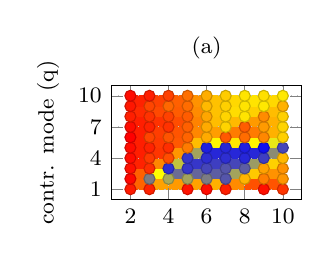
\begin{tikzpicture}
\begin{axis}
[
width=0.33\textwidth,
height=0.25\textwidth,
style={font=\footnotesize},
grid=major,
grid style={dotted},
align=center,
%xlabel={tensor order},
ylabel={contr. mode (q)},
title={{(a)}}, %  bgemm, asymmetric
scaled ticks=false,
zlabel={GFlops},
view={0}{90}, 
ytick={1,4,7,10},
xtick={2,4,6,8,10},
xmin=1, xmax=11,
ymin=0, ymax=11,
try min ticks=8,
zmin=300, zmax=2300,
point meta min=300, point meta max=2300,
colormap/hot, 
samples=50,
%colorbar sampled,
%colorbar/width=0.2cm,
%colorbar style={
%	point meta min=300, point meta max=2300,
%	samples=50,
%	font=\footnotesize,
%	ytick={300,1300,2300},
%	yticklabels={0.3,1.3,2.3},
%	%title={\scriptsize Gflops},
%	%ylabel={\scriptsize Gflops},
%}
]
%\addplot3[mesh, scatter,samples=50,shader=interp]
%\addplot3[only marks, mesh, scatter,scatter src=z,samples=50,] % z buffer=sort, scatter src=z,
\addplot3[contour filled={number=100},scatter,shader=flat,samples=50]
%\addplot3+[mesh,scatter,shader=flat corner,samples=50, only marks, mark size=2]
coordinates{
	
(2.000,1.000,2142.734) (2.000,2.000,2241.014) (2.000,3.000,2205.546) (2.000,4.000,2226.263) (2.000,5.000,2232.877) (2.000,6.000,2281.816) (2.000,7.000,2222.317) (2.000,8.000,2122.831) (2.000,9.000,2166.437) (2.000,10.000,2231.354) 

(3.000,1.000,2104.803) (3.000,2.000,620.292) (3.000,3.000,2053.810) (3.000,4.000,1989.460) (3.000,5.000,2100.108) (3.000,6.000,1923.866) (3.000,7.000,2109.798) (3.000,8.000,2032.918) (3.000,9.000,1931.835) (3.000,10.000,2137.550) 

(4.000,1.000,2303.560) (4.000,2.000,742.055) (4.000,3.000,436.752) (4.000,4.000,1889.266) (4.000,5.000,2050.848) (4.000,6.000,1845.429) (4.000,7.000,2029.757) (4.000,8.000,1947.246) (4.000,9.000,1753.968) (4.000,10.000,1945.836) 

(5.000,1.000,2197.949) (5.000,2.000,727.736) (5.000,3.000,441.734) (5.000,4.000,458.055) (5.000,5.000,1643.657) (5.000,6.000,1763.676) (5.000,7.000,1793.195) (5.000,8.000,1799.906) (5.000,9.000,1726.622) (5.000,10.000,1710.693) 

(6.000,1.000,2225.857) (6.000,2.000,621.489) (6.000,3.000,489.438) (6.000,4.000,435.500) (6.000,5.000,386.554) (6.000,6.000,1410.907) (6.000,7.000,1419.437) (6.000,8.000,1428.795) (6.000,9.000,1330.280) (6.000,10.000,1386.923) 

(7.000,1.000,2137.668) (7.000,2.000,530.662) (7.000,3.000,532.587) (7.000,4.000,439.307) (7.000,5.000,400.923) (7.000,6.000,1835.402) (7.000,7.000,1186.143) (7.000,8.000,1195.514) (7.000,9.000,1211.432) (7.000,10.000,1230.143) 

(8.000,1.000,2411.000) (8.000,2.000,1340.829) (8.000,3.000,546.729) (8.000,4.000,405.255) (8.000,5.000,381.061) (8.000,6.000,1724.053) (8.000,7.000,1816.684) (8.000,8.000,1103.276) (8.000,9.000,1109.365) (8.000,10.000,1119.582) 

(9.000,1.000,2215.896) (9.000,2.000,1637.409) (9.000,3.000,1448.314) (9.000,4.000,477.752) (9.000,5.000,353.959) (9.000,6.000,1596.361) (9.000,7.000,1496.308) (9.000,8.000,1566.431) (9.000,9.000,1085.107) (9.000,10.000,1135.908) 

(10.000,1.000,2011.147) (10.000,2.000,1504.412) (10.000,3.000,1538.421) (10.000,4.000,1335.732) (10.000,5.000,483.993) (10.000,6.000,1202.734) (10.000,7.000,1197.316) (10.000,8.000,1213.834) (10.000,9.000,1362.208) (10.000,10.000,1087.708)


};
\end{axis}
\end{tikzpicture}
\hfill
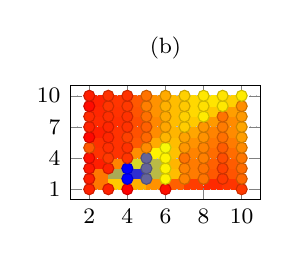
\begin{tikzpicture}
\begin{axis}
[
width=0.33\textwidth,
height=0.25\textwidth,
style={font=\footnotesize},
grid=major,
grid style={dotted},
align=center,
%xlabel={tensor order},
%ylabel={contr. mode (q)},
title={{(b)}}, %  ompfor<2d-slice> ttm<par-loops,seq-blas,$q$-slice>, asymmetric
scaled ticks=false,
zlabel={GFlops},
view={0}{90}, 
%view={-45}{45}, 
ytick={1,4,7,10},
xtick={2,4,6,8,10},
xmin=1, xmax=11,
ymin=0, ymax=11,
try min ticks=8,
zmin=300, zmax=2300,
point meta min=300, point meta max=2300,
colormap/hot, 
samples=50,
%colorbar sampled,
%colorbar/width=0.2cm,
%colorbar style={
%	point meta min=300, point meta max=2300,
%	samples=50,
%	font=\footnotesize,
%	ytick={300,1300,2300},
%	yticklabels={0.3,1.3,2.3},
%	%title={\scriptsize Gflops},
%	%ylabel={\scriptsize Gflops},
%}
]
%\addplot3[mesh, scatter,samples=50,shader=interp]
%\addplot3[only marks, mesh, scatter,scatter src=z,samples=50,] % z buffer=sort, scatter src=z,
\addplot3[contour filled={number=100},scatter,shader=flat,samples=50]
%\addplot3+[mesh,scatter,shader=flat corner,samples=50, only marks, mark size=2]
coordinates{

(2.000,1.000,2107.002) (2.000,2.000,2127.162) (2.000,3.000,2176.298) (2.000,4.000,2215.649) (2.000,5.000,1837.632) (2.000,6.000,2241.609) (2.000,7.000,2101.558) (2.000,8.000,2075.436) (2.000,9.000,2236.130) (2.000,10.000,2133.353) 

(3.000,1.000,2119.523) (3.000,2.000,167.437) (3.000,3.000,2112.420) (3.000,4.000,1989.285) (3.000,5.000,2041.921) (3.000,6.000,2084.201) (3.000,7.000,2080.454) (3.000,8.000,2046.614) (3.000,9.000,2013.009) (3.000,10.000,2024.421) 

(4.000,1.000,2285.299) (4.000,2.000,314.287) (4.000,3.000,311.849) (4.000,4.000,2011.869) (4.000,5.000,2039.029) (4.000,6.000,1944.642) (4.000,7.000,2023.178) (4.000,8.000,2033.385) (4.000,9.000,1992.379) (4.000,10.000,2039.303) 

(5.000,1.000,2475.804) (5.000,2.000,568.291) (5.000,3.000,562.230) (5.000,4.000,562.587) (5.000,5.000,1564.667) (5.000,6.000,1756.890) (5.000,7.000,1791.524) (5.000,8.000,1712.024) (5.000,9.000,1626.887) (5.000,10.000,1695.764) 

(6.000,1.000,2218.038) (6.000,2.000,1025.980) (6.000,3.000,1034.039) (6.000,4.000,1026.350) (6.000,5.000,945.367) (6.000,6.000,1340.191) (6.000,7.000,1422.937) (6.000,8.000,1402.244) (6.000,9.000,1375.707) (6.000,10.000,1411.432) 

(7.000,1.000,2307.246) (7.000,2.000,1602.074) (7.000,3.000,1617.348) (7.000,4.000,1682.539) (7.000,5.000,1516.443) (7.000,6.000,1446.511) (7.000,7.000,1229.353) (7.000,8.000,1202.606) (7.000,9.000,1245.855) (7.000,10.000,1211.880) 

(8.000,1.000,2441.539) (8.000,2.000,1699.771) (8.000,3.000,1686.405) (8.000,4.000,1622.372) (8.000,5.000,1600.438) (8.000,6.000,1530.707) (8.000,7.000,1508.466) (8.000,8.000,1073.808) (8.000,9.000,1123.363) (8.000,10.000,1096.486) 

(9.000,1.000,2330.060) (9.000,2.000,1985.056) (9.000,3.000,1941.312) (9.000,4.000,1892.533) (9.000,5.000,1805.699) (9.000,6.000,1706.515) (9.000,7.000,1658.818) (9.000,8.000,1693.350) (9.000,9.000,1093.684) (9.000,10.000,1112.530) 

(10.000,1.000,1988.818) (10.000,2.000,1750.516) (10.000,3.000,1728.226) (10.000,4.000,1678.568) (10.000,5.000,1576.395) (10.000,6.000,1476.492) (10.000,7.000,1429.733) (10.000,8.000,1496.574) (10.000,9.000,1557.162) (10.000,10.000,1068.719) 


};
\end{axis}
\end{tikzpicture}
\hfill
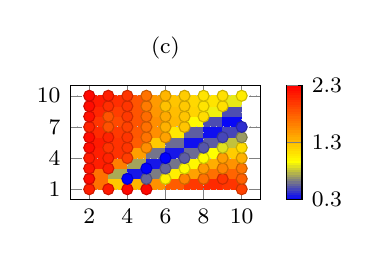
\begin{tikzpicture}
\begin{axis}
[
width=0.33\textwidth,
height=0.25\textwidth,
style={font=\footnotesize},
grid=major,
grid style={dotted},
align=center,
%xlabel={tensor order},
%ylabel={contr. mode (q)},
title={{(c)}}, %  ompfor<qd-slice> ttm<par-loops,seq-blas,$q$-slice>, asymmetric
scaled ticks=false,
zlabel={GFlops},
view={0}{90}, 
%view={-45}{45}, 
ytick={1,4,7,10},
xtick={2,4,6,8,10},
%xmin=2, xmax=10,
%ymin=1, ymax=10,
xmin=1, xmax=11,
ymin=0, ymax=11,
try min ticks=8,
zmin=300, zmax=2300,
point meta min=300, point meta max=2300,
%colormap/jet, 
colormap/hot, 
%colormap/blackwhite,
%colormap={whiteblack}{indices of colormap={\pgfplotscolormaplastindexof{blackwhite},...,0 of blackwhite}},
samples=50,
%colormap access=piecewise const,
colorbar sampled,
colorbar/width=0.2cm,
colorbar style={
	point meta min=300, point meta max=2300,
	samples=50,
	font=\footnotesize,
	ytick={300,1300,2300},
	yticklabels={0.3,1.3,2.3},
	%title={\scriptsize Gflops},
	%ylabel={\scriptsize Gflops},
}
]
%\addplot3[mesh, scatter,samples=50,shader=interp]
%\addplot3[only marks, mesh, scatter,scatter src=z,samples=50,] % z buffer=sort, scatter src=z,
\addplot3[contour filled={number=100},scatter,shader=flat,samples=50]
%\addplot3+[mesh,scatter,shader=flat corner,samples=50, only marks, mark size=2]
coordinates{

(2.000,1.000,2134.021) (2.000,2.000,2224.864) (2.000,3.000,2184.477) (2.000,4.000,2142.541) (2.000,5.000,2229.439) (2.000,6.000,2238.772) (2.000,7.000,2105.091) (2.000,8.000,2201.214) (2.000,9.000,2232.448) (2.000,10.000,2240.926) 

(3.000,1.000,2146.896) (3.000,2.000,167.544) (3.000,3.000,2121.476) (3.000,4.000,2105.304) (3.000,5.000,2027.717) (3.000,6.000,2104.722) (3.000,7.000,1866.561) (3.000,8.000,1855.180) (3.000,9.000,2041.894) (3.000,10.000,2122.692) 

(4.000,1.000,2244.985) (4.000,2.000,313.766) (4.000,3.000,167.879) (4.000,4.000,1973.457) (4.000,5.000,2013.391) (4.000,6.000,2010.678) (4.000,7.000,1949.136) (4.000,8.000,1989.844) (4.000,9.000,2017.192) (4.000,10.000,2015.899) 

(5.000,1.000,2250.694) (5.000,2.000,574.277) (5.000,3.000,315.908) (5.000,4.000,166.343) (5.000,5.000,1559.782) (5.000,6.000,1688.138) (5.000,7.000,1711.412) (5.000,8.000,1721.389) (5.000,9.000,1653.587) (5.000,10.000,1691.902) 

(6.000,1.000,2403.465) (6.000,2.000,1026.371) (6.000,3.000,576.699) (6.000,4.000,312.020) (6.000,5.000,160.917) (6.000,6.000,1443.174) (6.000,7.000,1370.699) (6.000,8.000,1414.204) (6.000,9.000,1283.900) (6.000,10.000,1351.446) 

(7.000,1.000,2305.894) (7.000,2.000,1613.830) (7.000,3.000,988.435) (7.000,4.000,554.792) (7.000,5.000,290.305) (7.000,6.000,157.356) (7.000,7.000,1270.432) (7.000,8.000,1266.914) (7.000,9.000,1255.620) (7.000,10.000,1224.914) 

(8.000,1.000,2437.239) (8.000,2.000,1706.219) (8.000,3.000,1489.110) (8.000,4.000,999.755) (8.000,5.000,531.137) (8.000,6.000,280.182) (8.000,7.000,148.892) (8.000,8.000,1156.621) (8.000,9.000,1110.478) (8.000,10.000,1116.944) 

(9.000,1.000,2355.395) (9.000,2.000,2003.839) (9.000,3.000,1603.752) (9.000,4.000,1477.309) (9.000,5.000,887.839) (9.000,6.000,492.554) (9.000,7.000,262.294) (9.000,8.000,150.408) (9.000,9.000,1129.997) (9.000,10.000,1121.143) 

(10.000,1.000,1944.959) (10.000,2.000,1789.054) (10.000,3.000,1665.441) (10.000,4.000,1375.291) (10.000,5.000,1147.731) (10.000,6.000,715.205) (10.000,7.000,422.658) (10.000,8.000,236.076) (10.000,9.000,136.520) (10.000,10.000,1078.495) 


};
\end{axis}
\end{tikzpicture}


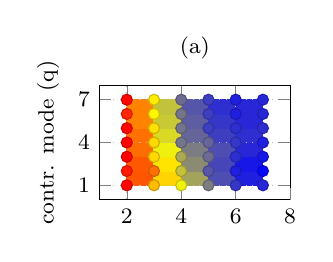
\begin{tikzpicture}
\begin{axis}
[
width=0.33\textwidth,
height=0.25\textwidth,
style={font=\footnotesize},
grid=major,
grid style={dotted},
align=center,
%xlabel={tensor order},
ylabel={contr. mode (q)},
title={{(a)}}, %  bgemm, asymmetric
scaled ticks=false,
zlabel={GFlops},
view={0}{90}, 
ytick={1,4,7,10},
xtick={2,4,6,8},
xmin=1, xmax=8,
ymin=0, ymax=8,
try min ticks=8,
zmin=0, zmax=2600,
point meta min=0, point meta max=2600,
colormap/hot, 
samples=50,
%colorbar sampled,
%colorbar/width=0.2cm,
%colorbar style={
%	point meta min=300, point meta max=2300,
%	samples=50,
%	font=\footnotesize,
%	ytick={300,1300,2300},
%	yticklabels={0.3,1.3,2.3},
%	%title={\scriptsize Gflops},
%	%ylabel={\scriptsize Gflops},
%}
]
%\addplot3[mesh, scatter,samples=50,shader=interp]
%\addplot3[only marks, mesh, scatter,scatter src=z,samples=50,] % z buffer=sort, scatter src=z,
\addplot3[contour filled={number=100},scatter,shader=flat,samples=50]
%\addplot3+[mesh,scatter,shader=flat corner,samples=50, only marks, mark size=2]
coordinates{

(2.000,1.000,2527.923) (2.000,2.000,2398.051) (2.000,3.000,2573.521) (2.000,4.000,2570.296) (2.000,5.000,2540.651) (2.000,6.000,2326.903) (2.000,7.000,2545.629) 

(3.000,1.000,1312.517) (3.000,2.000,1835.211) (3.000,3.000,1133.124) (3.000,4.000,1120.384) (3.000,5.000,1066.704) (3.000,6.000,915.932) (3.000,7.000,997.168) 

(4.000,1.000,825.045) (4.000,2.000,655.270) (4.000,3.000,579.750) (4.000,4.000,390.794) (4.000,5.000,411.134) (4.000,6.000,409.619) (4.000,7.000,375.457) 

(5.000,1.000,420.343) (5.000,2.000,308.678) (5.000,3.000,377.118) (5.000,4.000,348.232) (5.000,5.000,216.877) (5.000,6.000,232.073) (5.000,7.000,218.457) 

(6.000,1.000,206.774) (6.000,2.000,119.299) (6.000,3.000,167.691) (6.000,4.000,183.571) (6.000,5.000,179.989) (6.000,6.000,126.876) (6.000,7.000,128.135) 

(7.000,1.000,150.823) (7.000,2.000,33.170) (7.000,3.000,83.979) (7.000,4.000,128.221) (7.000,5.000,157.368) (7.000,6.000,143.557) (7.000,7.000,133.647) 


};
\end{axis}
\end{tikzpicture}
\hfill
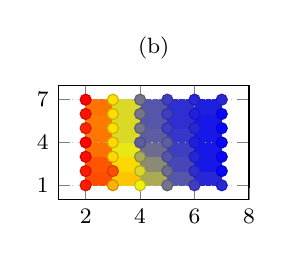
\begin{tikzpicture}
\begin{axis}
[
width=0.33\textwidth,
height=0.25\textwidth,
style={font=\footnotesize},
grid=major,
grid style={dotted},
align=center,
%xlabel={tensor order},
%ylabel={contr. mode (q)},
title={{(b)}}, %  ompfor<2d-slice> ttm<par-loops,seq-blas,$q$-slice>, asymmetric
scaled ticks=false,
zlabel={GFlops},
view={0}{90}, 
%view={-45}{45}, 
ytick={1,4,7,10},
xtick={2,4,6,8},
xmin=1, xmax=8,
ymin=0, ymax=8,
try min ticks=8,
zmin=0, zmax=2600,
point meta min=0, point meta max=2600,
colormap/hot, 
samples=50,
%colorbar sampled,
%colorbar/width=0.2cm,
%colorbar style={
%	point meta min=300, point meta max=2300,
%	samples=50,
%	font=\footnotesize,
%	ytick={300,1300,2300},
%	yticklabels={0.3,1.3,2.3},
%	%title={\scriptsize Gflops},
%	%ylabel={\scriptsize Gflops},
%}
]
%\addplot3[mesh, scatter,samples=50,shader=interp]
%\addplot3[only marks, mesh, scatter,scatter src=z,samples=50,] % z buffer=sort, scatter src=z,
\addplot3[contour filled={number=100},scatter,shader=flat,samples=50]
%\addplot3+[mesh,scatter,shader=flat corner,samples=50, only marks, mark size=2]
coordinates{

(2.000,1.000,2394.429) (2.000,2.000,2411.386) (2.000,3.000,2508.441) (2.000,4.000,2549.390) (2.000,5.000,2334.831) (2.000,6.000,2454.725) (2.000,7.000,2556.685) 

(3.000,1.000,1395.054) (3.000,2.000,2055.946) (3.000,3.000,1121.102) (3.000,4.000,1120.659) (3.000,5.000,1089.377) (3.000,6.000,1102.959) (3.000,7.000,1078.957) 

(4.000,1.000,819.991) (4.000,2.000,729.342) (4.000,3.000,579.869) (4.000,4.000,334.133) (4.000,5.000,390.153) (4.000,6.000,407.045) (4.000,7.000,394.057) 

(5.000,1.000,414.803) (5.000,2.000,369.532) (5.000,3.000,295.077) (5.000,4.000,318.473) (5.000,5.000,209.139) (5.000,6.000,214.825) (5.000,7.000,223.888) 

(6.000,1.000,208.097) (6.000,2.000,156.950) (6.000,3.000,141.868) (6.000,4.000,119.992) (6.000,5.000,134.757) (6.000,6.000,126.271) (6.000,7.000,133.034) 

(7.000,1.000,151.228) (7.000,2.000,27.225) (7.000,3.000,30.634) (7.000,4.000,31.221) (7.000,5.000,30.322) (7.000,6.000,31.152) (7.000,7.000,133.496) 


};
\end{axis}
\end{tikzpicture}
\hfill
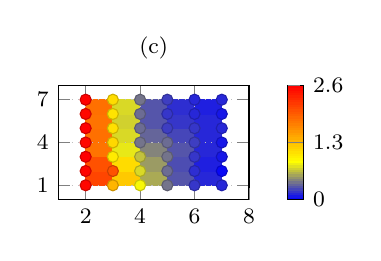
\begin{tikzpicture}
\begin{axis}
[
width=0.33\textwidth,
height=0.25\textwidth,
style={font=\footnotesize},
grid=major,
grid style={dotted},
align=center,
%xlabel={tensor order},
%ylabel={contr. mode (q)},
title={{(c)}}, %  ompfor<qd-slice> ttm<par-loops,seq-blas,$q$-slice>, asymmetric
scaled ticks=false,
zlabel={GFlops},
view={0}{90}, 
ytick={1,4,7,10},
xtick={2,4,6,8},
xmin=1, xmax=8,
ymin=0, ymax=8,
try min ticks=8,
zmin=0, zmax=2600,
point meta min=0, point meta max=2600,
%colormap/jet, 
colormap/hot, 
%colormap/blackwhite,
%colormap={whiteblack}{indices of colormap={\pgfplotscolormaplastindexof{blackwhite},...,0 of blackwhite}},
samples=50,
%colormap access=piecewise const,
colorbar sampled,
colorbar/width=0.2cm,
colorbar style={
point meta min=0, point meta max=2600,
samples=50,
font=\footnotesize,
ytick={0,1300,2600},
yticklabels={0,1.3,2.6},
%title={\scriptsize Gflops},
%ylabel={\scriptsize Gflops},
}
]
%\addplot3[mesh, scatter,samples=50,shader=interp]
%\addplot3[only marks, mesh, scatter,scatter src=z,samples=50,] % z buffer=sort, scatter src=z,
\addplot3[contour filled={number=100},scatter,shader=flat,samples=50]
%\addplot3+[mesh,scatter,shader=flat corner,samples=50, only marks, mark size=2]
coordinates{

(2.000,1.000,2536.639) (2.000,2.000,2549.050) (2.000,3.000,2598.729) (2.000,4.000,2525.744) (2.000,5.000,2590.830) (2.000,6.000,2544.134) (2.000,7.000,2589.762) 

(3.000,1.000,1375.656) (3.000,2.000,2048.636) (3.000,3.000,1013.687) (3.000,4.000,1124.134) (3.000,5.000,1075.977) (3.000,6.000,1052.382) (3.000,7.000,1098.544) 

(4.000,1.000,833.978) (4.000,2.000,732.322) (4.000,3.000,660.833) (4.000,4.000,413.827) (4.000,5.000,368.029) (4.000,6.000,382.244) (4.000,7.000,404.286) 

(5.000,1.000,415.086) (5.000,2.000,368.007) (5.000,3.000,411.465) (5.000,4.000,371.633) (5.000,5.000,212.971) (5.000,6.000,198.100) (5.000,7.000,222.798) 

(6.000,1.000,206.159) (6.000,2.000,156.941) (6.000,3.000,192.783) (6.000,4.000,217.075) (6.000,5.000,186.601) (6.000,6.000,132.454) (6.000,7.000,130.229) 

(7.000,1.000,150.869) (7.000,2.000,27.399) (7.000,3.000,91.695) (7.000,4.000,85.698) (7.000,5.000,132.060) (7.000,6.000,86.740) (7.000,7.000,146.783) 


};
\end{axis}
\end{tikzpicture}

\caption{%
\footnotesize %
Performance maps in double-precision Tflops of the proposed algorithms with varying tensor orders $p$  and contraction modes $q$. 
Tensors are asymmetrically-shaped on the upper plots and symmetrically-shaped on the lower plots.
In (a) and (d) function \tf{<gemm\_batch>} is executed,
in (b) and (e) \tf{<par-loops,seq-gemm>} with tensor slices, %
in (c) and (f) \tf{<par-loops,seq-gemm>} with subtensors.
\label{performance.tlib.contour}
}
\end{figure*}


\begin{figure*}[t]
\centering
%\tikzset{every mark/.append style={scale=1.5}}
\begin{tikzpicture}
\begin{axis}[
height=0.3\textheight,
width=0.49\textwidth,
style={font=\footnotesize},
grid=major,
grid style={dotted},
align=center,
xlabel={Tflops/s},
ylabel={Cumulative Probability},
ylabel near ticks,
%title={Empirical CDF},
xtick={0,200,400,600,800,1000,1200},
xticklabels={0,0.2,0.4,0.6,0.8,1.0,1.2},
ytick={0,0.25,0.5,0.75,1},
yticklabels={0,0.25,0.5,0.75,1},
mark repeat={16},
cycle list name=my exotic tlib case8
]
\addplot
coordinates{(255.725,0.000) (255.725,0.004) (259.197,0.009) (260.053,0.013) (261.586,0.018) (266.569,0.022) (266.569,0.027) (272.340,0.031) (273.829,0.036) (275.720,0.040) (279.751,0.045) (282.740,0.049) (283.254,0.054) (288.248,0.058) (299.073,0.062) (299.093,0.067) (299.121,0.071) (299.196,0.076) (300.283,0.080) (308.959,0.085) (311.773,0.089) (313.578,0.094) (319.080,0.098) (319.866,0.103) (324.231,0.107) (328.240,0.112) (330.141,0.116) (330.965,0.121) (331.324,0.125) (333.125,0.129) (334.131,0.134) (334.954,0.138) (335.269,0.143) (337.797,0.147) (339.578,0.152) (341.231,0.156) (342.026,0.161) (348.853,0.165) (349.914,0.170) (350.121,0.174) (350.382,0.179) (350.719,0.183) (351.459,0.188) (351.611,0.192) (353.682,0.196) (355.212,0.201) (358.899,0.205) (360.009,0.210) (360.079,0.214) (361.376,0.219) (362.121,0.223) (365.922,0.228) (367.431,0.232) (369.824,0.237) (370.284,0.241) (371.754,0.246) (373.873,0.250) (375.272,0.254) (376.335,0.259) (376.356,0.263) (378.550,0.268) (384.636,0.272) (390.014,0.277) (393.879,0.281) (402.543,0.286) (403.291,0.290) (405.389,0.295) (419.036,0.299) (420.826,0.304) (422.925,0.308) (433.035,0.312) (441.841,0.317) (444.146,0.321) (447.448,0.326) (448.331,0.330) (452.294,0.335) (459.688,0.339) (462.422,0.344) (463.678,0.348) (465.154,0.353) (467.339,0.357) (468.930,0.362) (471.164,0.366) (478.474,0.371) (484.753,0.375) (484.753,0.379) (549.371,0.384) (562.055,0.388) (565.716,0.393) (565.716,0.397) (566.285,0.402) (578.342,0.406) (579.356,0.411) (590.776,0.415) (590.776,0.420) (597.328,0.424) (605.817,0.429) (606.980,0.433) (607.225,0.437) (608.544,0.442) (609.297,0.446) (610.823,0.451) (610.823,0.455) (611.815,0.460) (613.232,0.464) (614.065,0.469) (614.600,0.473) (615.642,0.478) (616.110,0.482) (618.961,0.487) (621.699,0.491) (621.699,0.496) (621.833,0.500) (623.063,0.504) (625.010,0.509) (626.577,0.513) (626.577,0.518) (628.579,0.522) (629.842,0.527) (629.842,0.531) (632.055,0.536) (634.275,0.540) (638.210,0.545) (641.663,0.549) (668.783,0.554) (687.564,0.558) (687.924,0.562) (688.469,0.567) (688.481,0.571) (688.875,0.576) (692.222,0.580) (698.936,0.585) (705.324,0.589) (713.936,0.594) (713.936,0.598) (714.441,0.603) (717.570,0.607) (718.161,0.612) (720.706,0.616) (722.716,0.621) (722.716,0.625) (729.597,0.629) (739.345,0.634) (739.975,0.638) (741.589,0.643) (742.985,0.647) (743.868,0.652) (749.090,0.656) (749.121,0.661) (756.987,0.665) (757.437,0.670) (758.400,0.674) (761.521,0.679) (769.833,0.683) (773.767,0.688) (778.523,0.692) (786.813,0.696) (787.463,0.701) (789.226,0.705) (794.808,0.710) (796.961,0.714) (797.934,0.719) (799.552,0.723) (800.815,0.728) (801.397,0.732) (803.221,0.737) (803.221,0.741) (818.611,0.746) (821.626,0.750) (821.626,0.754) (831.468,0.759) (832.110,0.763) (832.110,0.768) (832.202,0.772) (832.202,0.777) (833.371,0.781) (833.371,0.786) (833.563,0.790) (833.563,0.795) (834.295,0.799) (835.646,0.804) (835.646,0.808) (840.780,0.812) (841.960,0.817) (841.960,0.821) (842.811,0.826) (848.447,0.830) (848.986,0.835) (849.574,0.839) (855.935,0.844) (859.296,0.848) (859.662,0.853) (859.662,0.857) (860.312,0.862) (860.312,0.866) (869.563,0.871) (869.563,0.875) (871.285,0.879) (871.285,0.884) (872.170,0.888) (875.218,0.893) (875.388,0.897) (877.362,0.902) (878.200,0.906) (878.200,0.911) (879.798,0.915) (879.798,0.920) (883.810,0.924) (889.482,0.929) (889.943,0.933) (896.800,0.937) (902.896,0.942) (908.473,0.946) (914.919,0.951) (918.687,0.955) (926.791,0.960) (928.500,0.964) (936.302,0.969) (939.220,0.973) (969.904,0.978) (995.783,0.982) (1000.624,0.987) (1016.770,0.991) (1034.495,0.996) (1039.696,1.000) };
%\label{coord:gemm_batch}
\addplot
coordinates{(132.897,0.000) (132.897,0.004) (136.068,0.009) (136.068,0.013) (137.742,0.018) (137.884,0.022) (143.498,0.027) (144.955,0.031) (295.083,0.036) (295.083,0.040) (320.062,0.045) (331.604,0.049) (331.604,0.054) (337.300,0.058) (343.392,0.062) (343.794,0.067) (345.733,0.071) (346.062,0.076) (346.960,0.080) (347.361,0.085) (358.377,0.089) (414.626,0.094) (422.328,0.098) (464.048,0.103) (464.048,0.107) (472.584,0.112) (473.238,0.116) (473.238,0.121) (479.780,0.125) (481.013,0.129) (482.579,0.134) (483.146,0.138) (486.033,0.143) (486.067,0.147) (486.067,0.152) (489.371,0.156) (493.390,0.161) (493.986,0.165) (496.473,0.170) (499.949,0.174) (500.090,0.179) (503.353,0.183) (506.701,0.188) (509.237,0.192) (509.332,0.196) (510.244,0.201) (512.394,0.205) (514.244,0.210) (517.174,0.214) (517.174,0.219) (518.479,0.223) (519.181,0.228) (519.262,0.232) (524.803,0.237) (526.706,0.241) (527.079,0.246) (528.095,0.250) (528.218,0.254) (533.786,0.259) (534.435,0.263) (536.302,0.268) (537.671,0.272) (539.606,0.277) (540.682,0.281) (540.918,0.286) (543.337,0.290) (544.287,0.295) (546.192,0.299) (546.768,0.304) (548.094,0.308) (550.870,0.312) (553.217,0.317) (555.172,0.321) (555.213,0.326) (555.213,0.330) (555.834,0.335) (555.884,0.339) (557.670,0.344) (560.171,0.348) (562.066,0.353) (563.140,0.357) (564.429,0.362) (565.598,0.366) (567.739,0.371) (567.739,0.375) (568.045,0.379) (568.932,0.384) (569.109,0.388) (569.625,0.393) (569.629,0.397) (569.629,0.402) (570.319,0.406) (571.665,0.411) (571.752,0.415) (572.203,0.420) (573.619,0.424) (574.866,0.429) (577.854,0.433) (578.777,0.437) (579.743,0.442) (580.489,0.446) (582.922,0.451) (585.846,0.455) (586.532,0.460) (586.532,0.464) (586.553,0.469) (588.012,0.473) (590.729,0.478) (591.671,0.482) (593.398,0.487) (594.018,0.491) (594.881,0.496) (598.932,0.500) (599.110,0.504) (599.110,0.509) (599.119,0.513) (599.939,0.518) (600.609,0.522) (600.612,0.527) (600.720,0.531) (601.750,0.536) (605.029,0.540) (605.855,0.545) (608.645,0.549) (608.645,0.554) (608.655,0.558) (609.150,0.562) (610.464,0.567) (610.464,0.571) (611.686,0.576) (612.931,0.580) (614.753,0.585) (615.460,0.589) (616.886,0.594) (616.961,0.598) (617.841,0.603) (619.059,0.607) (619.769,0.612) (620.182,0.616) (620.182,0.621) (621.057,0.625) (626.234,0.629) (626.770,0.634) (632.681,0.638) (635.248,0.643) (637.358,0.647) (638.793,0.652) (645.922,0.656) (646.566,0.661) (647.759,0.665) (653.497,0.670) (659.612,0.674) (667.091,0.679) (676.128,0.683) (689.957,0.688) (689.957,0.692) (692.090,0.696) (693.644,0.701) (694.942,0.705) (695.208,0.710) (696.511,0.714) (700.752,0.719) (700.752,0.723) (704.529,0.728) (707.088,0.732) (709.171,0.737) (710.664,0.741) (716.394,0.746) (717.806,0.750) (718.224,0.754) (718.224,0.759) (720.394,0.763) (722.171,0.768) (731.221,0.772) (741.327,0.777) (741.607,0.781) (743.307,0.786) (746.915,0.790) (750.340,0.795) (750.463,0.799) (751.232,0.804) (756.143,0.808) (761.653,0.812) (761.653,0.817) (770.584,0.821) (773.181,0.826) (778.548,0.830) (779.726,0.835) (780.614,0.839) (780.614,0.844) (782.530,0.848) (784.551,0.853) (795.813,0.857) (796.357,0.862) (800.700,0.866) (803.345,0.871) (803.512,0.875) (803.512,0.879) (807.562,0.884) (812.809,0.888) (814.100,0.893) (815.384,0.897) (816.274,0.902) (817.694,0.906) (826.678,0.911) (826.678,0.915) (833.236,0.920) (833.236,0.924) (833.826,0.929) (837.186,0.933) (838.316,0.937) (842.846,0.942) (844.404,0.946) (844.626,0.951) (845.073,0.955) (846.218,0.960) (846.218,0.964) (853.024,0.969) (853.065,0.973) (853.216,0.978) (853.256,0.982) (861.362,0.987) (870.434,0.991) (871.130,0.996) (877.689,1.000) };
%\label{coord:seq_loops_par_gemm_slice}
\addplot
coordinates{(247.352,0.000) (247.352,0.004) (249.133,0.009) (250.808,0.013) (251.654,0.018) (251.720,0.022) (252.640,0.027) (254.061,0.031) (254.414,0.036) (331.637,0.040) (337.772,0.045) (337.772,0.049) (339.426,0.054) (340.443,0.058) (345.104,0.062) (357.481,0.067) (448.340,0.071) (463.563,0.076) (464.506,0.080) (464.820,0.085) (468.185,0.089) (468.515,0.094) (472.461,0.098) (476.941,0.103) (477.966,0.107) (478.494,0.112) (478.901,0.116) (482.126,0.121) (483.687,0.125) (483.738,0.129) (493.474,0.134) (494.193,0.138) (496.551,0.143) (570.311,0.147) (570.311,0.152) (571.060,0.156) (572.724,0.161) (579.951,0.165) (583.516,0.170) (583.516,0.174) (587.734,0.179) (608.388,0.183) (619.407,0.188) (627.169,0.192) (635.447,0.196) (646.815,0.201) (671.147,0.205) (719.417,0.210) (722.525,0.214) (726.008,0.219) (742.956,0.223) (751.693,0.228) (767.475,0.232) (767.475,0.237) (768.327,0.241) (777.826,0.246) (779.988,0.250) (783.232,0.254) (794.709,0.259) (796.089,0.263) (796.955,0.268) (799.956,0.272) (801.911,0.277) (803.305,0.281) (803.430,0.286) (805.652,0.290) (806.341,0.295) (811.218,0.299) (811.503,0.304) (815.263,0.308) (816.284,0.312) (816.854,0.317) (820.276,0.321) (824.164,0.326) (824.397,0.330) (825.189,0.335) (827.757,0.339) (828.298,0.344) (831.274,0.348) (836.813,0.353) (841.188,0.357) (843.636,0.362) (846.284,0.366) (846.414,0.371) (846.634,0.375) (847.708,0.379) (850.987,0.384) (852.849,0.388) (853.853,0.393) (854.707,0.397) (855.188,0.402) (856.039,0.406) (860.951,0.411) (860.951,0.415) (861.226,0.420) (863.534,0.424) (864.601,0.429) (866.165,0.433) (869.267,0.437) (870.680,0.442) (870.870,0.446) (871.211,0.451) (871.211,0.455) (873.365,0.460) (873.425,0.464) (873.434,0.469) (874.751,0.473) (874.979,0.478) (876.361,0.482) (876.508,0.487) (876.732,0.491) (876.794,0.496) (878.357,0.500) (879.397,0.504) (880.678,0.509) (880.678,0.513) (888.447,0.518) (889.518,0.522) (891.371,0.527) (891.371,0.531) (894.807,0.536) (897.176,0.540) (907.935,0.545) (908.667,0.549) (909.843,0.554) (909.843,0.558) (911.298,0.562) (915.210,0.567) (916.777,0.571) (917.082,0.576) (917.082,0.580) (926.339,0.585) (931.164,0.589) (931.299,0.594) (931.299,0.598) (933.838,0.603) (933.838,0.607) (934.391,0.612) (934.391,0.616) (935.998,0.621) (937.507,0.625) (938.494,0.629) (938.693,0.634) (941.152,0.638) (941.152,0.643) (941.468,0.647) (943.132,0.652) (943.248,0.656) (947.615,0.661) (949.721,0.665) (957.884,0.670) (960.731,0.674) (962.085,0.679) (962.085,0.683) (965.869,0.688) (965.869,0.692) (967.799,0.696) (967.837,0.701) (968.171,0.705) (973.067,0.710) (974.058,0.714) (974.766,0.719) (974.835,0.723) (980.907,0.728) (986.498,0.732) (988.416,0.737) (989.720,0.741) (993.242,0.746) (995.211,0.750) (995.211,0.754) (996.017,0.759) (996.017,0.763) (996.226,0.768) (997.207,0.772) (1002.644,0.777) (1003.142,0.781) (1003.301,0.786) (1003.502,0.790) (1004.974,0.795) (1007.719,0.799) (1009.066,0.804) (1009.324,0.808) (1012.517,0.812) (1014.745,0.817) (1014.745,0.821) (1016.610,0.826) (1017.101,0.830) (1018.253,0.835) (1020.301,0.839) (1021.387,0.844) (1021.498,0.848) (1021.539,0.853) (1021.539,0.857) (1022.802,0.862) (1022.830,0.866) (1024.417,0.871) (1028.491,0.875) (1028.491,0.879) (1033.829,0.884) (1034.794,0.888) (1035.168,0.893) (1036.888,0.897) (1041.495,0.902) (1041.495,0.906) (1042.474,0.911) (1043.124,0.915) (1045.309,0.920) (1047.456,0.924) (1052.842,0.929) (1053.010,0.933) (1054.333,0.937) (1054.333,0.942) (1060.484,0.946) (1061.095,0.951) (1065.766,0.955) (1065.766,0.960) (1067.855,0.964) (1068.606,0.969) (1069.342,0.973) (1080.841,0.978) (1083.141,0.982) (1083.794,0.987) (1084.410,0.991) (1091.057,0.996) (1098.338,1.000) };
%\label{coord:par_loops_seq_gemm_slice}%
%\addplot
%coordinates{(233.348,0.000) (233.348,0.004) (246.744,0.009) (249.242,0.013) (252.439,0.018) (253.062,0.022) (253.062,0.027) (253.820,0.031) (254.414,0.036) (335.244,0.040) (339.393,0.045) (339.393,0.049) (342.447,0.054) (347.684,0.058) (353.586,0.062) (354.561,0.067) (399.462,0.071) (427.634,0.076) (454.801,0.080) (455.316,0.085) (457.886,0.089) (473.684,0.094) (479.239,0.098) (480.208,0.103) (480.927,0.107) (483.290,0.112) (485.297,0.116) (488.741,0.121) (490.083,0.125) (492.223,0.129) (493.400,0.134) (494.175,0.138) (494.282,0.143) (495.393,0.147) (566.938,0.152) (566.938,0.156) (568.505,0.161) (586.209,0.165) (591.691,0.170) (593.407,0.174) (594.118,0.179) (594.118,0.183) (603.401,0.188) (609.385,0.192) (622.177,0.196) (626.269,0.201) (639.496,0.205) (645.679,0.210) (659.602,0.214) (659.686,0.219) (679.703,0.223) (713.818,0.228) (714.799,0.232) (740.703,0.237) (761.600,0.241) (764.334,0.246) (766.553,0.250) (766.970,0.254) (770.375,0.259) (772.707,0.263) (776.026,0.268) (776.026,0.272) (776.876,0.277) (790.178,0.281) (790.178,0.286) (793.992,0.290) (794.928,0.295) (796.054,0.299) (797.878,0.304) (800.366,0.308) (802.113,0.312) (802.820,0.317) (803.501,0.321) (803.694,0.326) (810.397,0.330) (812.442,0.335) (813.443,0.339) (813.705,0.344) (815.494,0.348) (822.724,0.353) (826.509,0.357) (827.228,0.362) (828.441,0.366) (828.898,0.371) (831.226,0.375) (834.029,0.379) (842.320,0.384) (842.984,0.388) (843.032,0.393) (843.706,0.397) (844.209,0.402) (845.195,0.406) (845.469,0.411) (850.295,0.415) (852.719,0.420) (854.103,0.424) (855.564,0.429) (857.649,0.433) (858.737,0.437) (862.653,0.442) (864.704,0.446) (864.704,0.451) (866.669,0.455) (868.193,0.460) (868.957,0.464) (869.834,0.469) (870.761,0.473) (872.157,0.478) (872.298,0.482) (872.813,0.487) (876.421,0.491) (876.799,0.496) (876.828,0.500) (878.056,0.504) (878.662,0.509) (883.027,0.513) (884.117,0.518) (892.007,0.522) (894.486,0.527) (894.486,0.531) (896.589,0.536) (897.894,0.540) (899.459,0.545) (899.459,0.549) (899.530,0.554) (899.633,0.558) (901.996,0.562) (905.641,0.567) (906.892,0.571) (908.199,0.576) (910.256,0.580) (920.572,0.585) (920.957,0.589) (925.593,0.594) (925.593,0.598) (927.180,0.603) (930.176,0.607) (932.234,0.612) (937.210,0.616) (937.210,0.621) (938.725,0.625) (941.093,0.629) (941.093,0.634) (954.658,0.638) (956.436,0.643) (957.306,0.647) (959.220,0.652) (962.240,0.656) (962.240,0.661) (962.589,0.665) (963.008,0.670) (964.511,0.674) (964.511,0.679) (967.591,0.683) (972.499,0.688) (972.624,0.692) (974.736,0.696) (975.202,0.701) (991.913,0.705) (992.940,0.710) (993.123,0.714) (994.406,0.719) (995.981,0.723) (996.096,0.728) (996.207,0.732) (996.207,0.737) (996.848,0.741) (996.848,0.746) (998.366,0.750) (1000.430,0.754) (1001.429,0.759) (1003.002,0.763) (1006.193,0.768) (1006.193,0.772) (1007.943,0.777) (1011.845,0.781) (1011.845,0.786) (1014.223,0.790) (1014.386,0.795) (1016.185,0.799) (1018.993,0.804) (1022.949,0.808) (1025.253,0.812) (1026.343,0.817) (1026.343,0.821) (1028.065,0.826) (1028.065,0.830) (1028.096,0.835) (1035.043,0.839) (1035.559,0.844) (1035.863,0.848) (1035.863,0.853) (1036.255,0.857) (1040.914,0.862) (1042.122,0.866) (1042.454,0.871) (1045.099,0.875) (1045.956,0.879) (1045.956,0.884) (1046.194,0.888) (1046.700,0.893) (1048.146,0.897) (1051.096,0.902) (1051.151,0.906) (1052.661,0.911) (1054.889,0.915) (1056.999,0.920) (1056.999,0.924) (1060.709,0.929) (1060.961,0.933) (1060.961,0.937) (1061.053,0.942) (1061.053,0.946) (1061.361,0.951) (1065.605,0.955) (1073.460,0.960) (1074.982,0.964) (1076.513,0.969) (1078.500,0.973) (1088.390,0.978) (1089.961,0.982) (1090.352,0.987) (1090.403,0.991) (1112.107,0.996) (1131.842,1.000) };
%%\label{coord:par_loops_par_gemm_slice}%
\addplot
coordinates{(139.045,0.000) (139.045,0.004) (159.874,0.009) (177.233,0.013) (219.289,0.018) (232.646,0.022) (232.646,0.027) (250.312,0.031) (312.060,0.036) (317.756,0.040) (335.426,0.045) (344.136,0.049) (345.807,0.054) (347.401,0.058) (354.547,0.062) (356.930,0.067) (407.347,0.071) (407.347,0.076) (411.281,0.080) (411.281,0.085) (429.429,0.089) (460.629,0.094) (460.629,0.098) (464.336,0.103) (465.809,0.107) (465.852,0.112) (467.102,0.116) (467.102,0.121) (477.009,0.125) (482.486,0.129) (484.672,0.134) (484.969,0.138) (487.104,0.143) (492.104,0.147) (496.217,0.152) (499.393,0.156) (499.393,0.161) (509.526,0.165) (512.006,0.170) (515.005,0.174) (516.981,0.179) (517.675,0.183) (517.968,0.188) (520.373,0.192) (520.677,0.196) (521.961,0.201) (523.654,0.205) (524.834,0.210) (527.562,0.214) (527.788,0.219) (529.480,0.223) (529.775,0.228) (530.153,0.232) (530.153,0.237) (530.312,0.241) (533.496,0.246) (533.580,0.250) (535.723,0.254) (536.107,0.259) (537.720,0.263) (538.579,0.268) (540.861,0.272) (544.477,0.277) (545.307,0.281) (545.608,0.286) (547.931,0.290) (547.931,0.295) (547.973,0.299) (549.355,0.304) (549.715,0.308) (549.729,0.312) (550.298,0.317) (551.102,0.321) (552.274,0.326) (554.311,0.330) (555.861,0.335) (556.443,0.339) (557.652,0.344) (557.705,0.348) (557.989,0.353) (561.628,0.357) (562.214,0.362) (567.162,0.366) (569.626,0.371) (569.626,0.375) (570.088,0.379) (570.163,0.384) (570.429,0.388) (572.824,0.393) (572.928,0.397) (573.086,0.402) (574.462,0.406) (580.283,0.411) (581.922,0.415) (586.086,0.420) (586.668,0.424) (586.692,0.429) (586.996,0.433) (587.843,0.437) (588.351,0.442) (589.585,0.446) (590.255,0.451) (590.596,0.455) (591.287,0.460) (592.872,0.464) (593.032,0.469) (593.751,0.473) (595.031,0.478) (595.443,0.482) (597.258,0.487) (597.568,0.491) (598.281,0.496) (600.474,0.500) (601.965,0.504) (602.583,0.509) (607.657,0.513) (612.036,0.518) (613.147,0.522) (614.121,0.527) (614.756,0.531) (614.784,0.536) (615.118,0.540) (615.129,0.545) (625.125,0.549) (628.308,0.554) (629.591,0.558) (642.127,0.562) (647.202,0.567) (649.356,0.571) (661.798,0.576) (662.874,0.580) (667.975,0.585) (678.384,0.589) (686.612,0.594) (693.161,0.598) (693.570,0.603) (694.483,0.607) (699.176,0.612) (702.971,0.616) (705.968,0.621) (706.345,0.625) (724.478,0.629) (724.478,0.634) (726.909,0.638) (732.057,0.643) (740.123,0.647) (741.643,0.652) (747.244,0.656) (747.306,0.661) (750.741,0.665) (755.102,0.670) (756.329,0.674) (757.233,0.679) (758.487,0.683) (758.789,0.688) (759.596,0.692) (759.835,0.696) (761.985,0.701) (761.985,0.705) (769.256,0.710) (769.256,0.714) (772.204,0.719) (772.204,0.723) (773.111,0.728) (773.111,0.732) (778.113,0.737) (778.113,0.741) (778.632,0.746) (778.632,0.750) (781.807,0.754) (784.444,0.759) (784.917,0.763) (785.417,0.768) (792.785,0.772) (792.785,0.777) (794.971,0.781) (805.235,0.786) (808.642,0.790) (811.980,0.795) (814.204,0.799) (814.842,0.804) (814.842,0.808) (816.068,0.812) (816.068,0.817) (820.250,0.821) (824.139,0.826) (829.333,0.830) (830.376,0.835) (841.479,0.839) (841.705,0.844) (843.290,0.848) (843.290,0.853) (844.255,0.857) (847.920,0.862) (847.920,0.866) (848.080,0.871) (848.591,0.875) (848.591,0.879) (848.939,0.884) (849.419,0.888) (855.330,0.893) (855.330,0.897) (856.603,0.902) (862.321,0.906) (863.912,0.911) (863.912,0.915) (867.650,0.920) (868.830,0.924) (869.867,0.929) (877.180,0.933) (880.426,0.937) (881.277,0.942) (886.586,0.946) (888.091,0.951) (888.123,0.955) (888.565,0.960) (891.050,0.964) (895.526,0.969) (898.723,0.973) (905.589,0.978) (907.406,0.982) (911.298,0.987) (914.998,0.991) (920.793,0.996) (937.256,1.000) };
%\label{coord:seq_loops_par_gemm_subtensor}
\addplot
coordinates{(88.913,0.000) (88.913,0.004) (121.560,0.009) (124.334,0.013) (124.500,0.018) (125.141,0.022) (125.268,0.027) (125.441,0.031) (125.917,0.036) (125.925,0.040) (165.698,0.045) (201.603,0.049) (205.172,0.054) (218.915,0.058) (226.989,0.062) (235.089,0.067) (235.089,0.071) (235.959,0.076) (236.116,0.080) (236.351,0.085) (237.898,0.089) (237.912,0.094) (237.920,0.098) (237.920,0.103) (239.527,0.107) (239.527,0.112) (239.880,0.116) (239.880,0.121) (239.914,0.125) (240.792,0.129) (241.713,0.134) (241.867,0.138) (243.090,0.143) (243.608,0.147) (243.608,0.152) (243.762,0.156) (243.774,0.161) (243.774,0.165) (244.756,0.170) (244.875,0.174) (244.905,0.179) (245.701,0.183) (245.701,0.188) (245.967,0.192) (245.967,0.196) (246.618,0.201) (247.058,0.205) (247.531,0.210) (247.834,0.214) (248.133,0.219) (248.847,0.223) (249.447,0.228) (249.527,0.232) (250.225,0.237) (250.447,0.241) (251.396,0.246) (251.495,0.250) (251.609,0.254) (251.778,0.259) (251.892,0.263) (251.954,0.268) (251.989,0.272) (252.012,0.277) (252.715,0.281) (254.041,0.286) (254.654,0.290) (271.445,0.295) (271.445,0.299) (303.328,0.304) (340.460,0.308) (351.839,0.312) (367.856,0.317) (375.532,0.321) (375.532,0.326) (392.663,0.330) (410.418,0.335) (425.807,0.339) (427.792,0.344) (439.829,0.348) (439.829,0.353) (445.785,0.357) (449.121,0.362) (449.443,0.366) (449.443,0.371) (450.439,0.375) (451.768,0.379) (454.632,0.384) (457.631,0.388) (457.946,0.393) (459.828,0.397) (461.835,0.402) (461.835,0.406) (464.586,0.411) (464.586,0.415) (464.941,0.420) (464.941,0.424) (465.130,0.429) (465.630,0.433) (467.664,0.437) (468.653,0.442) (469.463,0.446) (472.054,0.451) (472.054,0.455) (473.123,0.460) (474.015,0.464) (474.522,0.469) (474.758,0.473) (474.758,0.478) (476.518,0.482) (476.565,0.487) (476.836,0.491) (476.836,0.496) (477.178,0.500) (477.533,0.504) (478.905,0.509) (482.626,0.513) (485.179,0.518) (487.715,0.522) (489.961,0.527) (492.910,0.531) (493.880,0.536) (499.400,0.540) (507.905,0.545) (562.000,0.549) (602.103,0.554) (609.940,0.558) (616.745,0.562) (647.953,0.567) (678.936,0.571) (679.723,0.576) (682.864,0.580) (683.186,0.585) (704.021,0.589) (704.021,0.594) (705.294,0.598) (722.295,0.603) (729.372,0.607) (744.590,0.612) (744.829,0.616) (751.461,0.621) (761.434,0.625) (761.434,0.629) (766.051,0.634) (767.283,0.638) (767.283,0.643) (774.390,0.647) (777.663,0.652) (777.663,0.656) (778.124,0.661) (781.517,0.665) (782.803,0.670) (790.133,0.674) (797.809,0.679) (801.194,0.683) (802.003,0.688) (802.279,0.692) (802.744,0.696) (803.404,0.701) (803.404,0.705) (819.404,0.710) (819.494,0.714) (822.267,0.719) (825.749,0.723) (825.944,0.728) (826.270,0.732) (826.868,0.737) (828.757,0.741) (829.276,0.746) (833.540,0.750) (834.840,0.754) (846.001,0.759) (850.413,0.763) (851.250,0.768) (853.819,0.772) (854.550,0.777) (862.009,0.781) (862.422,0.786) (862.652,0.790) (862.652,0.795) (863.780,0.799) (864.180,0.804) (865.813,0.808) (869.759,0.812) (872.591,0.817) (874.129,0.821) (877.332,0.826) (878.625,0.830) (880.391,0.835) (887.842,0.839) (888.632,0.844) (898.937,0.848) (900.391,0.853) (907.983,0.857) (909.039,0.862) (915.175,0.866) (916.538,0.871) (917.097,0.875) (938.477,0.879) (940.597,0.884) (944.494,0.888) (947.192,0.893) (970.923,0.897) (972.814,0.902) (973.734,0.906) (985.312,0.911) (996.363,0.915) (1005.662,0.920) (1010.992,0.924) (1011.410,0.929) (1025.932,0.933) (1028.218,0.937) (1036.753,0.942) (1046.596,0.946) (1051.857,0.951) (1053.456,0.955) (1056.594,0.960) (1062.795,0.964) (1063.635,0.969) (1071.527,0.973) (1072.652,0.978) (1074.841,0.982) (1077.415,0.987) (1097.273,0.991) (1100.214,0.996) (1137.087,1.000) };
%\label{coord:par_loops_seq_gemm_subtensor}%
%\addplot
%coordinates{(88.639,0.000) (88.639,0.004) (122.870,0.009) (124.864,0.013) (124.875,0.018) (125.562,0.022) (125.739,0.027) (125.753,0.031) (125.766,0.036) (126.247,0.040) (166.549,0.045) (202.180,0.049) (206.964,0.054) (216.655,0.058) (223.629,0.062) (223.629,0.067) (227.041,0.071) (234.310,0.076) (237.227,0.080) (237.355,0.085) (237.389,0.089) (238.875,0.094) (239.021,0.098) (239.768,0.103) (240.238,0.107) (240.899,0.112) (240.899,0.116) (241.272,0.121) (241.608,0.125) (241.608,0.129) (241.953,0.134) (242.334,0.138) (242.840,0.143) (243.932,0.147) (244.079,0.152) (244.190,0.156) (244.195,0.161) (244.195,0.165) (244.237,0.170) (244.339,0.174) (244.420,0.179) (244.459,0.183) (244.459,0.188) (245.571,0.192) (245.571,0.196) (245.806,0.201) (245.806,0.205) (245.878,0.210) (245.941,0.214) (246.069,0.219) (246.210,0.223) (246.210,0.228) (246.256,0.232) (246.453,0.237) (247.250,0.241) (247.892,0.246) (248.290,0.250) (248.507,0.254) (249.122,0.259) (250.230,0.263) (250.237,0.268) (250.350,0.272) (251.404,0.277) (251.516,0.281) (253.726,0.286) (254.135,0.290) (275.759,0.295) (275.759,0.299) (315.976,0.304) (320.573,0.308) (357.659,0.312) (369.749,0.317) (369.749,0.321) (373.890,0.326) (420.094,0.330) (421.147,0.335) (426.981,0.339) (431.468,0.344) (432.419,0.348) (449.541,0.353) (450.477,0.357) (450.532,0.362) (451.577,0.366) (454.910,0.371) (458.670,0.375) (458.670,0.379) (459.906,0.384) (461.593,0.388) (461.831,0.393) (461.831,0.397) (462.979,0.402) (462.979,0.406) (465.037,0.411) (465.037,0.415) (466.040,0.420) (467.892,0.424) (467.892,0.429) (469.399,0.433) (469.934,0.437) (471.489,0.442) (471.489,0.446) (471.853,0.451) (472.965,0.455) (473.338,0.460) (476.292,0.464) (476.328,0.469) (476.367,0.473) (477.354,0.478) (477.971,0.482) (477.971,0.487) (479.584,0.491) (480.385,0.496) (480.437,0.500) (480.629,0.504) (484.704,0.509) (488.280,0.513) (494.840,0.518) (494.944,0.522) (495.436,0.527) (535.537,0.531) (554.955,0.536) (555.149,0.540) (555.149,0.545) (579.700,0.549) (604.103,0.554) (604.103,0.558) (626.485,0.562) (642.714,0.567) (647.910,0.571) (657.903,0.576) (706.559,0.580) (717.599,0.585) (726.178,0.589) (726.909,0.594) (741.473,0.598) (741.473,0.603) (755.950,0.607) (761.694,0.612) (761.694,0.616) (771.155,0.621) (776.606,0.625) (778.156,0.629) (778.156,0.634) (779.892,0.638) (782.762,0.643) (783.835,0.647) (796.327,0.652) (796.752,0.656) (802.478,0.661) (806.760,0.665) (808.317,0.670) (810.215,0.674) (810.578,0.679) (812.436,0.683) (812.628,0.688) (824.910,0.692) (833.603,0.696) (835.124,0.701) (839.771,0.705) (840.193,0.710) (842.361,0.714) (842.904,0.719) (844.547,0.723) (844.547,0.728) (845.681,0.732) (850.891,0.737) (851.087,0.741) (852.784,0.746) (853.790,0.750) (855.162,0.754) (856.976,0.759) (857.032,0.763) (858.079,0.768) (859.494,0.772) (860.481,0.777) (860.954,0.781) (865.913,0.786) (866.870,0.790) (867.081,0.795) (867.081,0.799) (867.544,0.804) (869.190,0.808) (871.757,0.812) (872.267,0.817) (873.829,0.821) (876.689,0.826) (881.338,0.830) (886.954,0.835) (892.347,0.839) (895.631,0.844) (897.000,0.848) (898.473,0.853) (900.277,0.857) (913.004,0.862) (916.032,0.866) (920.491,0.871) (929.178,0.875) (934.892,0.879) (948.188,0.884) (951.511,0.888) (957.366,0.893) (962.552,0.897) (973.781,0.902) (982.030,0.906) (985.431,0.911) (986.979,0.915) (991.721,0.920) (1001.269,0.924) (1007.658,0.929) (1015.481,0.933) (1016.348,0.937) (1020.479,0.942) (1039.124,0.946) (1047.262,0.951) (1050.128,0.955) (1050.819,0.960) (1064.074,0.964) (1064.561,0.969) (1072.954,0.973) (1074.442,0.978) (1081.525,0.982) (1091.827,0.987) (1097.833,0.991) (1101.829,0.996) (1104.746,1.000) };
%\label{coord:par_loops_par_gemm_subtensor}
\end{axis}
\end{tikzpicture}
\hfill
\begin{tikzpicture}
\begin{axis}[
height=0.3\textheight,
width=0.49\textwidth,
style={font=\footnotesize},
grid=major,
grid style={dotted},
align=center,
xlabel={Tflops/s},
ylabel={Cumulative Probability},
ylabel near ticks,
ytick={0,0.25,0.5,0.75,1},
yticklabels={0,0.25,0.5,0.75,1},
title={},
xtick={0,200,400,600,800},
xticklabels={0,0.2,0.4,0.6,0.8},
mark repeat={4},
cycle list name=my exotic tlib case8
]
\addplot
coordinates{(5.389,0.000) (5.389,0.011) (12.953,0.022) (16.535,0.033) (19.598,0.044) (22.425,0.056) (24.042,0.067) (27.210,0.078) (34.027,0.089) (37.994,0.100) (39.345,0.111) (40.258,0.122) (41.571,0.133) (42.192,0.144) (43.201,0.156) (59.423,0.167) (59.491,0.178) (60.316,0.189) (64.826,0.200) (66.507,0.211) (66.818,0.222) (68.883,0.233) (71.033,0.244) (71.595,0.256) (71.774,0.267) (73.466,0.278) (73.697,0.289) (73.839,0.300) (74.330,0.311) (75.174,0.322) (75.872,0.333) (78.119,0.344) (80.638,0.356) (81.265,0.367) (82.917,0.378) (83.075,0.389) (88.325,0.400) (89.373,0.411) (90.445,0.422) (91.080,0.433) (93.279,0.444) (93.873,0.456) (94.599,0.467) (96.042,0.478) (96.564,0.489) (99.032,0.500) (99.184,0.511) (100.439,0.522) (104.135,0.533) (108.342,0.544) (109.516,0.556) (111.386,0.567) (117.983,0.578) (123.277,0.589) (129.213,0.600) (130.064,0.611) (132.213,0.622) (137.890,0.633) (140.986,0.644) (147.071,0.656) (149.068,0.667) (151.479,0.678) (153.102,0.689) (155.072,0.700) (156.146,0.711) (162.244,0.722) (182.146,0.733) (185.791,0.744) (202.553,0.756) (216.699,0.767) (229.168,0.778) (260.054,0.789) (262.806,0.800) (263.037,0.811) (269.675,0.822) (279.343,0.833) (287.265,0.844) (291.458,0.856) (303.260,0.867) (314.948,0.878) (338.053,0.889) (347.261,0.900) (363.619,0.911) (385.352,0.922) (410.914,0.933) (419.956,0.944) (444.571,0.956) (508.791,0.967) (555.168,0.978) (592.434,0.989) (595.211,1.000) };
\label{coord:gemm_batch}
\addplot
coordinates{(2.480,0.000) (2.480,0.011) (2.506,0.022) (2.674,0.033) (3.136,0.044) (3.138,0.056) (3.176,0.067) (3.211,0.078) (3.232,0.089) (3.428,0.100) (3.592,0.111) (3.656,0.122) (3.713,0.133) (4.062,0.144) (4.175,0.156) (4.298,0.167) (4.352,0.178) (4.354,0.189) (4.757,0.200) (5.021,0.211) (5.066,0.222) (5.103,0.233) (5.309,0.244) (5.397,0.256) (5.470,0.267) (5.619,0.278) (5.631,0.289) (5.684,0.300) (6.049,0.311) (6.272,0.322) (6.324,0.333) (6.499,0.344) (6.877,0.356) (6.916,0.367) (7.137,0.378) (7.202,0.389) (7.205,0.400) (7.309,0.411) (7.438,0.422) (7.504,0.433) (7.870,0.444) (7.935,0.456) (8.021,0.467) (8.026,0.478) (8.052,0.489) (8.154,0.500) (8.335,0.511) (8.401,0.522) (8.430,0.533) (8.749,0.544) (8.774,0.556) (9.013,0.567) (9.091,0.578) (9.358,0.589) (10.113,0.600) (10.713,0.611) (10.738,0.622) (10.883,0.633) (11.215,0.644) (11.953,0.656) (14.214,0.667) (14.256,0.678) (14.432,0.689) (14.968,0.700) (15.708,0.711) (16.476,0.722) (17.515,0.733) (17.720,0.744) (19.410,0.756) (19.732,0.767) (20.105,0.778) (20.588,0.789) (20.959,0.800) (22.705,0.811) (24.038,0.822) (25.419,0.833) (25.741,0.844) (25.770,0.856) (28.691,0.867) (29.188,0.878) (29.891,0.889) (30.284,0.900) (32.135,0.911) (44.790,0.922) (56.718,0.933) (77.187,0.944) (91.345,0.956) (104.722,0.967) (118.410,0.978) (121.757,0.989) (131.545,1.000) };
\label{coord:seq_loops_par_gemm_slice}
\addplot
coordinates{(6.966,0.000) (6.966,0.011) (7.133,0.022) (7.173,0.033) (7.188,0.044) (8.278,0.056) (8.438,0.067) (8.448,0.078) (9.779,0.089) (11.225,0.100) (11.232,0.111) (11.482,0.122) (12.680,0.133) (14.313,0.144) (14.456,0.156) (14.470,0.167) (17.564,0.178) (17.876,0.189) (17.941,0.200) (18.181,0.211) (22.380,0.222) (22.448,0.233) (22.476,0.244) (22.552,0.256) (27.332,0.267) (27.435,0.278) (28.153,0.289) (28.405,0.300) (31.899,0.311) (31.920,0.322) (32.263,0.333) (34.659,0.344) (37.073,0.356) (37.365,0.367) (37.709,0.378) (38.260,0.389) (38.532,0.400) (41.366,0.411) (42.032,0.422) (43.655,0.433) (49.242,0.444) (49.544,0.456) (53.550,0.467) (54.271,0.478) (64.078,0.489) (66.658,0.500) (68.394,0.511) (80.306,0.522) (81.797,0.533) (82.786,0.544) (83.001,0.556) (83.393,0.567) (89.084,0.578) (91.151,0.589) (96.942,0.600) (106.699,0.611) (108.333,0.622) (109.405,0.633) (111.835,0.644) (115.006,0.656) (119.532,0.667) (119.969,0.678) (128.639,0.689) (134.215,0.700) (134.539,0.711) (143.462,0.722) (163.467,0.733) (172.469,0.744) (183.351,0.756) (193.910,0.767) (202.737,0.778) (219.610,0.789) (221.238,0.800) (244.492,0.811) (245.892,0.822) (253.536,0.833) (259.795,0.844) (273.855,0.856) (276.445,0.867) (288.377,0.878) (305.261,0.889) (316.211,0.900) (327.961,0.911) (401.734,0.922) (440.257,0.933) (474.227,0.944) (507.993,0.956) (595.182,0.967) (652.655,0.978) (703.573,0.989) (738.594,1.000) };
\label{coord:par_loops_seq_gemm_slice}%
%\addplot
%coordinates{(7.209,0.000) (7.209,0.011) (7.211,0.022) (7.260,0.033) (7.265,0.044) (8.242,0.056) (8.399,0.067) (8.452,0.078) (10.049,0.089) (11.214,0.100) (11.263,0.111) (11.393,0.122) (13.448,0.133) (14.335,0.144) (14.353,0.156) (14.456,0.167) (17.324,0.178) (17.797,0.189) (17.888,0.200) (18.194,0.211) (22.289,0.222) (22.403,0.233) (22.421,0.244) (22.502,0.256) (27.328,0.267) (27.366,0.278) (28.123,0.289) (28.339,0.300) (31.967,0.311) (32.182,0.322) (32.231,0.333) (34.628,0.344) (37.160,0.356) (37.782,0.367) (38.385,0.378) (38.674,0.389) (38.832,0.400) (41.370,0.411) (44.284,0.422) (44.462,0.433) (49.550,0.444) (49.873,0.456) (54.731,0.467) (55.000,0.478) (64.284,0.489) (68.624,0.500) (68.931,0.511) (80.394,0.522) (82.593,0.533) (82.801,0.544) (83.194,0.556) (83.435,0.567) (89.248,0.578) (90.879,0.589) (96.741,0.600) (107.583,0.611) (109.511,0.622) (110.630,0.633) (111.719,0.644) (115.436,0.656) (119.821,0.667) (120.065,0.678) (128.575,0.689) (134.027,0.700) (134.647,0.711) (144.055,0.722) (162.815,0.733) (171.684,0.744) (183.300,0.756) (190.918,0.767) (201.949,0.778) (218.761,0.789) (220.159,0.800) (244.522,0.811) (245.282,0.822) (258.446,0.833) (272.801,0.844) (273.012,0.856) (288.211,0.867) (304.617,0.878) (316.156,0.889) (328.405,0.900) (368.228,0.911) (401.698,0.922) (439.725,0.933) (473.508,0.944) (507.719,0.956) (597.989,0.967) (646.502,0.978) (702.690,0.989) (743.473,1.000) };
%%\label{coord:par_loops_par_gemm_slice}%
\addplot
coordinates{(3.188,0.000) (3.188,0.011) (3.595,0.022) (4.375,0.033) (4.946,0.044) (5.513,0.056) (5.616,0.067) (6.109,0.078) (6.417,0.089) (6.441,0.100) (6.463,0.111) (6.495,0.122) (7.202,0.133) (7.290,0.144) (7.373,0.156) (7.976,0.167) (8.308,0.178) (8.778,0.189) (8.811,0.200) (9.346,0.211) (9.358,0.222) (10.274,0.233) (10.805,0.244) (11.162,0.256) (11.359,0.267) (11.641,0.278) (11.988,0.289) (14.153,0.300) (14.444,0.311) (15.528,0.322) (16.073,0.333) (16.379,0.344) (16.453,0.356) (17.567,0.367) (18.568,0.378) (19.502,0.389) (19.766,0.400) (20.681,0.411) (20.868,0.422) (22.607,0.433) (24.281,0.444) (25.077,0.456) (25.632,0.467) (27.262,0.478) (29.172,0.489) (30.239,0.500) (30.299,0.511) (32.272,0.522) (32.338,0.533) (35.011,0.544) (37.575,0.556) (39.725,0.567) (40.362,0.578) (41.346,0.589) (42.813,0.600) (42.881,0.611) (42.963,0.622) (43.025,0.633) (47.947,0.644) (49.509,0.656) (49.603,0.667) (51.294,0.678) (52.471,0.689) (56.444,0.700) (57.380,0.711) (58.485,0.722) (62.427,0.733) (64.716,0.744) (67.883,0.756) (67.957,0.767) (74.517,0.778) (75.687,0.789) (77.405,0.800) (78.134,0.811) (84.410,0.822) (93.148,0.833) (95.186,0.844) (104.092,0.856) (108.171,0.867) (110.657,0.878) (113.504,0.889) (117.451,0.900) (122.058,0.911) (123.706,0.922) (124.113,0.933) (133.297,0.944) (143.987,0.956) (169.652,0.967) (225.167,0.978) (243.015,0.989) (257.326,1.000) };
\label{coord:seq_loops_par_gemm_subtensor}
\addplot
coordinates{(7.206,0.000) (7.206,0.011) (9.973,0.022) (13.491,0.033) (17.587,0.044) (22.245,0.056) (28.080,0.067) (34.567,0.078) (37.543,0.089) (39.550,0.100) (41.266,0.111) (47.878,0.122) (48.840,0.133) (49.581,0.144) (53.959,0.156) (58.881,0.167) (60.809,0.178) (61.744,0.189) (64.119,0.200) (64.256,0.211) (64.371,0.222) (64.427,0.233) (66.351,0.244) (68.402,0.256) (69.488,0.267) (70.416,0.278) (72.361,0.289) (73.624,0.300) (75.323,0.311) (75.783,0.322) (76.464,0.333) (79.210,0.344) (80.150,0.356) (82.683,0.367) (83.077,0.378) (83.902,0.389) (84.853,0.400) (85.018,0.411) (85.862,0.422) (88.196,0.433) (89.691,0.444) (90.364,0.456) (96.788,0.467) (97.671,0.478) (99.701,0.489) (102.869,0.500) (106.090,0.511) (107.110,0.522) (111.811,0.533) (113.619,0.544) (119.893,0.556) (121.524,0.567) (124.738,0.578) (128.667,0.589) (130.891,0.600) (133.719,0.611) (139.194,0.622) (139.606,0.633) (143.679,0.644) (145.448,0.656) (146.543,0.667) (149.207,0.678) (155.383,0.689) (158.994,0.700) (162.475,0.711) (170.211,0.722) (190.528,0.733) (192.599,0.744) (219.255,0.756) (220.977,0.767) (244.742,0.778) (250.417,0.789) (251.188,0.800) (271.361,0.811) (287.024,0.822) (299.117,0.833) (305.826,0.844) (316.368,0.856) (320.921,0.867) (321.755,0.878) (328.677,0.889) (339.445,0.900) (367.429,0.911) (404.739,0.922) (440.162,0.933) (475.732,0.944) (509.031,0.956) (598.716,0.967) (657.022,0.978) (702.183,0.989) (742.380,1.000) };
\label{coord:par_loops_seq_gemm_subtensor}%
%\addplot
%coordinates{(7.212,0.000) (7.212,0.011) (10.011,0.022) (13.539,0.033) (17.378,0.044) (22.389,0.056) (28.106,0.067) (34.405,0.078) (40.508,0.089) (41.396,0.100) (48.261,0.111) (49.558,0.122) (50.170,0.133) (51.809,0.144) (57.811,0.156) (61.159,0.167) (62.097,0.178) (62.424,0.189) (62.450,0.200) (63.373,0.211) (64.682,0.222) (64.690,0.233) (66.579,0.244) (68.643,0.256) (70.318,0.267) (72.730,0.278) (73.089,0.289) (75.577,0.300) (75.873,0.311) (76.173,0.322) (79.537,0.333) (80.237,0.344) (81.660,0.356) (82.201,0.367) (82.620,0.378) (82.801,0.389) (84.592,0.400) (85.532,0.411) (87.975,0.422) (88.324,0.433) (89.836,0.444) (90.765,0.456) (96.818,0.467) (98.563,0.478) (100.473,0.489) (103.306,0.500) (106.110,0.511) (107.658,0.522) (111.771,0.533) (113.166,0.544) (120.032,0.556) (121.278,0.567) (123.413,0.578) (128.493,0.589) (130.675,0.600) (134.769,0.611) (138.160,0.622) (139.439,0.633) (144.066,0.644) (146.750,0.656) (147.590,0.667) (148.834,0.678) (155.493,0.689) (157.446,0.700) (164.070,0.711) (171.766,0.722) (191.534,0.733) (192.454,0.744) (220.404,0.756) (220.935,0.767) (243.383,0.778) (247.595,0.789) (252.160,0.800) (273.417,0.811) (288.048,0.822) (296.879,0.833) (306.454,0.844) (314.765,0.856) (319.523,0.867) (323.128,0.878) (329.499,0.889) (336.142,0.900) (367.449,0.911) (397.556,0.922) (439.901,0.933) (475.795,0.944) (509.080,0.956) (596.224,0.967) (657.014,0.978) (702.208,0.989) (743.527,1.000) };
%\label{coord:par_loops_par_gemm_subtensor}%
\end{axis}
\end{tikzpicture} % boxplot
\caption{ %
\footnotesize%
Cumulative performance distributions of the proposed algorithms for case eight.
Each distribution line belongs to one algorithm:
\tf{<gemm\_batch>} \ref{coord:gemm_batch} , %
\tf{<seq-loops,par-gemm>} (\ref{coord:seq_loops_par_gemm_slice}) and
\tf{<par-loops,seq-gemm>} (\ref{coord:par_loops_seq_gemm_slice}) using tensor slices,
\tf{<seq-loops,par-gemm>} (\ref{coord:seq_loops_par_gemm_subtensor}) and
\tf{<par-loops,seq-gemm>} (\ref{coord:par_loops_seq_gemm_subtensor}) using subtensors.
Tensors are asymmetrically (left plot) and symmetrically shaped (right plot).
}
\label{fig:performance.tlib.case8}
\end{figure*}


\begin{figure*}[t]
\begin{tikzpicture}
\begin{axis}[
boxplot/draw direction=y,
width=0.37\textwidth,
height=0.3\textheight,
style={font=\footnotesize},
grid=major,
grid style={dotted},
align=center,
xlabel={$k$-order layout},
ylabel={TFlops},
ylabel near ticks,
%title={Performance (Tflops/s)},
xtick={1,2,3,4,5,6,7},
xticklabels={1,2,3,4,5,6,7},
ymin=0,
ymax=200,
ytick={0,100,200},
yticklabels={0,0.1,0.2},
cycle list={{black}},
boxplot/variable width,
boxplot/box extend=0.5,
boxplot/every box/.style={fill=black,thick},
boxplot/every median/.style={draw=white,thin},
]
\addplot+[boxplot prepared={lower whisker = 12.953287, lower quartile = 60.316441, median = 75.006325, upper quartile = 89.433827, upper whisker = 117.121454} ] coordinates{};
\addplot+[boxplot prepared={lower whisker = 12.640045, lower quartile = 48.857803, median = 71.928801, upper quartile = 83.642690, upper whisker = 129.266128} ] coordinates{};
\addplot+[boxplot prepared={lower whisker = 11.285366, lower quartile = 38.052710, median = 47.911392, upper quartile = 58.133262, upper whisker = 82.945640} ] coordinates{};
\addplot+[boxplot prepared={lower whisker = 15.226172, lower quartile = 57.231846, median = 80.633181, upper quartile = 93.816564, upper whisker = 183.850079} ] coordinates{};
\addplot+[boxplot prepared={lower whisker = 14.986315, lower quartile = 49.549662, median = 65.947492, upper quartile = 82.637276, upper whisker = 134.213232} ] coordinates{};
\addplot+[boxplot prepared={lower whisker = 10.126218, lower quartile = 48.886168, median = 65.468008, upper quartile = 78.704242, upper whisker = 142.986427} ] coordinates{};
\addplot+[boxplot prepared={lower whisker = 9.920391, lower quartile = 46.556304, median = 53.812431, upper quartile = 67.449759, upper whisker = 97.531103} ] coordinates{};
\end{axis}
\end{tikzpicture}
\begin{tikzpicture}
\begin{axis}[
boxplot/draw direction=y,
width=0.37\textwidth,
height=0.3\textheight,
style={font=\footnotesize},
grid=major,
grid style={dotted},
align=center,
xlabel={$k$-order layout},
%xlabel={Function},
%ylabel={GFlops},
%ylabel near ticks,
%title={Performance (Tflops/s)},
xtick={1,2,3,4,5,6,7},
xticklabels={1,2,3,4,5,6,7},
ymin=0,
ymax=200,
ytick={0,100,200},
yticklabels={0,0.1,0.2},
cycle list={{black}},
boxplot/variable width,
boxplot/box extend=0.5,
boxplot/every box/.style={fill=black,thick},
boxplot/every median/.style={draw=white,thin},
]
\addplot+[boxplot prepared={lower whisker = 9.972735, lower quartile = 50.927006, median = 64.426586, upper quartile = 79.210059, upper whisker = 102.890428} ] coordinates{};
\addplot+[boxplot prepared={lower whisker = 9.924992, lower quartile = 53.823097, median = 66.585367, upper quartile = 76.424392, upper whisker = 126.976560} ] coordinates{};
\addplot+[boxplot prepared={lower whisker = 9.870402, lower quartile = 40.752707, median = 53.587394, upper quartile = 66.305725, upper whisker = 101.453234} ] coordinates{};
\addplot+[boxplot prepared={lower whisker = 14.708473, lower quartile = 68.924818, median = 80.163598, upper quartile = 97.636473, upper whisker = 172.275314} ] coordinates{};
\addplot+[boxplot prepared={lower whisker = 13.901132, lower quartile = 56.095772, median = 71.850410, upper quartile = 87.921333, upper whisker = 133.760673} ] coordinates{};
\addplot+[boxplot prepared={lower whisker = 9.637782, lower quartile = 64.849736, median = 77.669292, upper quartile = 95.936764, upper whisker = 142.318829} ] coordinates{};
\addplot+[boxplot prepared={lower whisker = 8.748652, lower quartile = 51.209701, median = 67.054182, upper quartile = 87.504879, upper whisker = 115.340741} ] coordinates{};
\end{axis}
\end{tikzpicture}
\begin{tikzpicture}
\begin{axis}[
boxplot/draw direction=y,
width=0.37\textwidth,
height=0.3\textheight,
style={font=\footnotesize},
grid=major,
grid style={dotted},
align=center,
xlabel={$k$-order layout},
%xlabel={Function},
%ylabel={Gflops},
%ylabel near ticks,
%title={},
xtick={1,2,3,4,5,6,7},
xticklabels={1,2,3,4,5,6,7},
ymin=0,
ymax=200,
ytick={0,100,200},
yticklabels={0,0.1,0.2},
cycle list={{black}},
boxplot/variable width,
boxplot/box extend=0.5,
boxplot/every box/.style={fill=black,thick},
boxplot/every median/.style={draw=white,thin},
]
\addplot+[boxplot prepared={lower whisker = 7.132722, lower quartile = 11.482166, median = 22.426546, upper quartile = 34.658759, upper whisker = 102.949746} ] coordinates{};
\addplot+[boxplot prepared={lower whisker = 6.479361, lower quartile = 14.151379, median = 27.103188, upper quartile = 40.479719, upper whisker = 97.896991} ] coordinates{};
\addplot+[boxplot prepared={lower whisker = 6.588109, lower quartile = 14.269192, median = 27.672456, upper quartile = 47.110864, upper whisker = 76.267702} ] coordinates{};
\addplot+[boxplot prepared={lower whisker = 10.384620, lower quartile = 19.559000, median = 36.409643, upper quartile = 56.801437, upper whisker = 115.192574} ] coordinates{};
\addplot+[boxplot prepared={lower whisker = 9.428007, lower quartile = 18.814353, median = 35.234564, upper quartile = 50.282299, upper whisker = 93.764754} ] coordinates{};
\addplot+[boxplot prepared={lower whisker = 8.495888, lower quartile = 18.190874, median = 34.228483, upper quartile = 68.448730, upper whisker = 110.241613} ] coordinates{};
\addplot+[boxplot prepared={lower whisker = 7.307545, lower quartile = 16.797509, median = 31.145092, upper quartile = 47.293157, upper whisker = 95.475018} ] coordinates{};
\end{axis}
\end{tikzpicture}
\caption{ %
\footnotesize%
Box plots visualizing performance statics in double-precision Tflops of a tensor-times-matrix algorithm for linear $k$-order tensor formats.
The algorithm loops over single-threaded \tf{gemm} with tensor slices with asymmetrically-shaped tensors on the left plot and with subtensors with symmetrically-shaped tensors on the right plot.
Box plot number $k$ denotes the utilized $k$-order storage.
}
\label{fig:performance.tlib.format}
\end{figure*}

\begin{figure*}[t]
\centering
\tikzset{every mark/.append style={scale=1.5}}
\begin{tikzpicture}
\begin{axis}[
height=0.3\textheight,
width=0.5\textwidth,
style={font=\footnotesize},
grid=major,
grid style={dotted},
align=center,
xlabel={Tflops/s},
ylabel={Cumulative Probability},
ylabel near ticks,
%title={Empirical CDF},
xtick={0,200,400,600,800,1000,1200},
xticklabels={0,0.2,0.4,0.6,0.8,1.0,1.2},
ytick={0,0.25,0.5,0.75,1},
yticklabels={0,0.25,0.5,0.75,1},
mark repeat={16},
cycle list name=my exotic compare 1,
]
\addplot%%+[const plo, line width=1,mark options={scale=2}]
coordinates{(126.866,0.000) (127.677,0.006) (128.446,0.012) (247.352,0.019) (250.808,0.025) (252.096,0.031) (254.061,0.037) (321.953,0.043) (337.772,0.049) (357.481,0.056) (412.844,0.062) (450.627,0.068) (455.588,0.074) (464.506,0.080) (468.515,0.086) (474.322,0.093) (477.948,0.099) (480.605,0.105) (482.078,0.111) (483.738,0.117) (487.720,0.123) (489.836,0.130) (492.948,0.136) (494.196,0.142) (499.662,0.148) (506.376,0.154) (510.779,0.160) (515.783,0.167) (520.894,0.173) (525.108,0.179) (527.089,0.185) (532.859,0.191) (538.446,0.198) (544.298,0.204) (551.766,0.210) (557.982,0.216) (563.185,0.222) (566.275,0.228) (570.012,0.235) (571.158,0.241) (576.303,0.247) (578.059,0.253) (579.951,0.259) (585.897,0.265) (590.075,0.272) (599.910,0.278) (626.566,0.284) (634.520,0.290) (646.815,0.296) (656.521,0.302) (661.127,0.309) (676.246,0.315) (688.133,0.321) (694.718,0.327) (699.650,0.333) (701.233,0.340) (712.888,0.346) (720.135,0.352) (725.611,0.358) (730.510,0.364) (733.161,0.370) (742.291,0.377) (745.256,0.383) (749.667,0.389) (752.126,0.395) (755.487,0.401) (758.905,0.407) (764.158,0.414) (765.321,0.420) (767.475,0.426) (768.327,0.432) (768.950,0.438) (772.050,0.444) (774.813,0.451) (776.982,0.457) (780.481,0.463) (782.098,0.469) (785.876,0.475) (792.372,0.481) (795.377,0.488) (796.955,0.494) (800.447,0.500) (803.250,0.506) (803.664,0.512) (806.341,0.519) (811.503,0.525) (816.284,0.531) (819.680,0.537) (824.874,0.543) (827.025,0.549) (829.100,0.556) (832.980,0.562) (836.813,0.568) (842.330,0.574) (843.940,0.580) (846.414,0.586) (848.632,0.593) (852.849,0.599) (854.707,0.605) (856.039,0.611) (859.563,0.617) (861.226,0.623) (866.165,0.630) (870.346,0.636) (870.870,0.642) (872.054,0.648) (873.365,0.654) (874.751,0.660) (876.361,0.667) (876.810,0.673) (877.733,0.679) (879.397,0.685) (880.678,0.691) (887.431,0.698) (889.518,0.704) (891.440,0.710) (893.903,0.716) (897.176,0.722) (904.337,0.728) (909.843,0.735) (914.883,0.741) (920.173,0.747) (923.853,0.753) (928.112,0.759) (931.755,0.765) (935.248,0.772) (936.845,0.778) (940.755,0.784) (941.951,0.790) (943.555,0.796) (946.601,0.802) (949.882,0.809) (957.884,0.815) (962.085,0.821) (965.307,0.827) (967.837,0.833) (974.058,0.840) (978.633,0.846) (983.465,0.852) (987.243,0.858) (993.242,0.864) (996.226,0.870) (1003.142,0.877) (1004.974,0.883) (1007.971,0.889) (1012.517,0.895) (1017.101,0.901) (1021.387,0.907) (1021.985,0.914) (1024.096,0.920) (1027.183,0.926) (1031.292,0.932) (1033.829,0.938) (1037.798,0.944) (1043.124,0.951) (1052.842,0.957) (1054.946,0.963) (1061.595,0.969) (1067.855,0.975) (1083.141,0.981) (1084.562,0.988) (1101.861,0.994) (1196.246,1.000) };
\label{coord:nonsymmetric.tlib.slice}
\addplot%%+[const plo %] %, line width=1,mark options={scale=2}]
coordinates{(39.550,0.000) (43.114,0.006) (70.346,0.012) (77.245,0.019) (79.570,0.025) (82.998,0.031) (114.998,0.037) (124.203,0.043) (139.879,0.049) (141.161,0.056) (141.686,0.062) (142.219,0.068) (161.072,0.074) (163.577,0.080) (174.279,0.086) (177.320,0.093) (178.717,0.099) (189.501,0.105) (193.508,0.111) (200.786,0.117) (204.520,0.123) (206.140,0.130) (207.206,0.136) (207.992,0.142) (214.557,0.148) (230.989,0.154) (235.636,0.160) (241.057,0.167) (244.729,0.173) (252.024,0.179) (255.686,0.185) (262.891,0.191) (266.307,0.198) (269.518,0.204) (271.184,0.210) (275.542,0.216) (280.687,0.222) (282.972,0.228) (286.782,0.235) (289.704,0.241) (291.724,0.247) (293.848,0.253) (295.234,0.259) (296.332,0.265) (297.270,0.272) (299.897,0.278) (302.580,0.284) (304.920,0.290) (306.456,0.296) (309.228,0.302) (312.951,0.309) (316.467,0.315) (318.262,0.321) (320.325,0.327) (323.732,0.333) (325.847,0.340) (327.659,0.346) (328.894,0.352) (331.488,0.358) (335.512,0.364) (338.491,0.370) (340.020,0.377) (346.111,0.383) (426.043,0.389) (432.175,0.395) (432.964,0.401) (433.759,0.407) (435.457,0.414) (436.158,0.420) (437.890,0.426) (444.750,0.432) (447.338,0.438) (455.131,0.444) (459.660,0.451) (464.654,0.457) (467.057,0.463) (474.215,0.469) (479.418,0.475) (481.156,0.481) (498.735,0.488) (501.447,0.494) (503.446,0.500) (504.986,0.506) (506.476,0.512) (507.895,0.519) (508.999,0.525) (510.054,0.531) (510.692,0.537) (512.411,0.543) (517.055,0.549) (518.668,0.556) (519.877,0.562) (520.706,0.568) (521.724,0.574) (523.148,0.580) (525.072,0.586) (527.088,0.593) (528.029,0.599) (528.514,0.605) (528.759,0.611) (529.588,0.617) (530.077,0.623) (530.762,0.630) (531.997,0.636) (532.778,0.642) (533.508,0.648) (533.947,0.654) (535.946,0.660) (536.735,0.667) (537.364,0.673) (538.118,0.679) (538.761,0.685) (539.418,0.691) (539.621,0.698) (540.086,0.704) (540.920,0.710) (541.705,0.716) (543.270,0.722) (544.178,0.728) (545.083,0.735) (545.682,0.741) (546.180,0.747) (546.887,0.753) (547.892,0.759) (549.700,0.765) (550.753,0.772) (551.629,0.778) (552.877,0.784) (554.315,0.790) (556.279,0.796) (557.919,0.802) (558.861,0.809) (560.317,0.815) (561.354,0.821) (564.021,0.827) (581.844,0.833) (588.241,0.840) (599.169,0.846) (604.501,0.852) (605.837,0.858) (611.346,0.864) (614.485,0.870) (618.627,0.877) (621.710,0.883) (624.989,0.889) (629.365,0.895) (635.038,0.901) (647.006,0.907) (657.583,0.914) (659.633,0.920) (661.884,0.926) (665.294,0.932) (668.252,0.938) (676.451,0.944) (679.661,0.951) (682.525,0.957) (693.310,0.963) (762.747,0.969) (772.635,0.975) (778.889,0.981) (798.965,0.988) (801.849,0.994) (812.196,1.000) };
\label{coord:nonsymmetric.tcl}
\addplot%%+[const plo %, line width=1,mark options={scale=2}]
coordinates{(225.666,0.000) (245.546,0.006) (251.857,0.012) (308.017,0.019) (320.236,0.025) (328.040,0.031) (330.465,0.037) (335.565,0.043) (340.689,0.049) (341.663,0.056) (346.282,0.062) (348.621,0.068) (350.505,0.074) (352.451,0.080) (353.014,0.086) (354.747,0.093) (356.749,0.099) (357.662,0.105) (358.948,0.111) (359.398,0.117) (360.653,0.123) (362.134,0.130) (362.583,0.136) (364.466,0.142) (365.263,0.148) (366.394,0.154) (367.236,0.160) (369.095,0.167) (370.649,0.173) (373.207,0.179) (373.564,0.185) (375.244,0.191) (376.006,0.198) (376.672,0.204) (378.452,0.210) (379.569,0.216) (380.310,0.222) (382.547,0.228) (384.196,0.235) (384.723,0.241) (386.180,0.247) (387.023,0.253) (387.320,0.259) (387.707,0.265) (388.128,0.272) (388.683,0.278) (389.504,0.284) (390.120,0.290) (391.187,0.296) (392.488,0.302) (393.816,0.309) (395.046,0.315) (397.090,0.321) (398.233,0.327) (399.301,0.333) (400.195,0.340) (400.850,0.346) (401.912,0.352) (402.635,0.358) (404.107,0.364) (404.997,0.370) (406.677,0.377) (406.980,0.383) (407.795,0.389) (407.831,0.395) (408.133,0.401) (409.897,0.407) (410.349,0.414) (410.648,0.420) (411.018,0.426) (411.560,0.432) (411.869,0.438) (412.260,0.444) (412.568,0.451) (413.224,0.457) (413.770,0.463) (413.909,0.469) (414.189,0.475) (414.335,0.481) (414.799,0.488) (415.123,0.494) (415.270,0.500) (415.644,0.506) (415.935,0.512) (416.203,0.519) (416.402,0.525) (416.736,0.531) (416.894,0.537) (417.341,0.543) (417.526,0.549) (417.984,0.556) (418.345,0.562) (418.756,0.568) (419.021,0.574) (419.900,0.580) (420.599,0.586) (421.253,0.593) (421.551,0.599) (422.684,0.605) (423.514,0.611) (423.835,0.617) (424.336,0.623) (424.463,0.630) (424.623,0.636) (425.859,0.642) (426.324,0.648) (427.562,0.654) (428.208,0.660) (429.116,0.667) (429.428,0.673) (431.560,0.679) (431.993,0.685) (432.269,0.691) (432.781,0.698) (435.552,0.704) (436.427,0.710) (438.954,0.716) (441.262,0.722) (441.955,0.728) (442.482,0.735) (445.076,0.741) (446.364,0.747) (446.720,0.753) (448.114,0.759) (448.594,0.765) (449.916,0.772) (450.869,0.778) (451.556,0.784) (452.329,0.790) (452.831,0.796) (454.060,0.802) (455.127,0.809) (455.447,0.815) (456.478,0.821) (457.412,0.827) (458.195,0.833) (458.752,0.840) (459.626,0.846) (460.996,0.852) (461.170,0.858) (461.791,0.864) (463.517,0.870) (464.558,0.877) (465.576,0.883) (466.713,0.889) (468.709,0.895) (470.663,0.901) (472.333,0.907) (474.872,0.914) (477.891,0.920) (483.193,0.926) (485.981,0.932) (506.884,0.938) (509.948,0.944) (525.788,0.951) (537.015,0.957) (538.682,0.963) (543.571,0.969) (546.662,0.975) (555.336,0.981) (557.484,0.988) (563.236,0.994) (571.135,1.000) };
\label{coord:nonsymmetric.tblis}
\addplot%%+[const plo %] %, line width=1,mark options={scale=2}]
coordinates{(95.840,0.000) (97.274,0.006) (101.815,0.012) (172.303,0.019) (176.090,0.025) (177.440,0.031) (189.410,0.037) (230.635,0.043) (236.036,0.049) (257.899,0.056) (266.170,0.062) (275.126,0.068) (279.649,0.074) (282.064,0.080) (306.943,0.086) (313.494,0.093) (316.812,0.099) (320.134,0.105) (328.615,0.111) (335.154,0.117) (344.168,0.123) (346.080,0.130) (348.220,0.136) (352.075,0.142) (356.279,0.148) (360.375,0.154) (362.058,0.160) (365.374,0.167) (368.370,0.173) (370.945,0.179) (373.472,0.185) (375.272,0.191) (383.855,0.198) (389.186,0.204) (394.008,0.210) (396.350,0.216) (398.014,0.222) (401.277,0.228) (403.433,0.235) (407.438,0.241) (410.873,0.247) (412.627,0.253) (414.717,0.259) (415.399,0.265) (418.953,0.272) (420.360,0.278) (421.496,0.284) (424.921,0.290) (427.062,0.296) (427.735,0.302) (428.246,0.309) (428.984,0.315) (430.352,0.321) (431.481,0.327) (432.142,0.333) (432.992,0.340) (435.309,0.346) (436.297,0.352) (437.536,0.358) (439.385,0.364) (441.739,0.370) (442.294,0.377) (445.981,0.383) (446.513,0.389) (447.625,0.395) (453.713,0.401) (454.220,0.407) (456.368,0.414) (459.768,0.420) (461.980,0.426) (467.078,0.432) (467.964,0.438) (468.650,0.444) (470.697,0.451) (473.554,0.457) (473.769,0.463) (477.155,0.469) (479.318,0.475) (480.250,0.481) (488.258,0.488) (492.532,0.494) (496.091,0.500) (499.316,0.506) (505.910,0.512) (515.365,0.519) (518.952,0.525) (520.328,0.531) (522.280,0.537) (524.142,0.543) (525.965,0.549) (527.471,0.556) (528.199,0.562) (529.174,0.568) (529.990,0.574) (530.817,0.580) (532.326,0.586) (533.889,0.593) (535.598,0.599) (536.342,0.605) (537.106,0.611) (538.110,0.617) (539.181,0.623) (542.987,0.630) (543.551,0.636) (544.443,0.642) (547.260,0.648) (550.666,0.654) (553.498,0.660) (554.841,0.667) (555.526,0.673) (557.562,0.679) (559.434,0.685) (564.584,0.691) (566.839,0.698) (568.357,0.704) (570.161,0.710) (571.553,0.716) (576.548,0.722) (578.298,0.728) (580.459,0.735) (583.103,0.741) (585.077,0.747) (586.828,0.753) (589.198,0.759) (590.278,0.765) (592.004,0.772) (592.853,0.778) (593.514,0.784) (594.006,0.790) (595.181,0.796) (595.630,0.802) (596.333,0.809) (596.725,0.815) (597.509,0.821) (599.064,0.827) (601.333,0.833) (602.925,0.840) (603.386,0.846) (604.066,0.852) (605.365,0.858) (606.921,0.864) (608.554,0.870) (610.795,0.877) (612.913,0.883) (619.902,0.889) (620.616,0.895) (621.809,0.901) (623.938,0.907) (626.662,0.914) (634.513,0.920) (638.052,0.926) (639.178,0.932) (640.047,0.938) (641.406,0.944) (642.168,0.951) (649.169,0.957) (651.481,0.963) (660.361,0.969) (666.032,0.975) (711.872,0.981) (718.484,0.988) (721.594,0.994) (736.497,1.000) };
\label{coord:nonsymmetric.libtorch}
\addplot%+[const plo %, line width=1,mark options={scale=2}]
coordinates{(98.208,0.000) (107.261,0.006) (112.468,0.012) (126.460,0.019) (143.066,0.025) (145.827,0.031) (146.079,0.037) (147.373,0.043) (151.233,0.049) (154.489,0.056) (156.317,0.062) (159.600,0.068) (161.695,0.074) (164.402,0.080) (166.588,0.086) (167.130,0.093) (167.976,0.099) (169.256,0.105) (171.563,0.111) (172.969,0.117) (174.338,0.123) (176.407,0.130) (177.493,0.136) (179.606,0.142) (181.200,0.148) (181.570,0.154) (182.068,0.160) (182.783,0.167) (184.021,0.173) (185.389,0.179) (186.755,0.185) (187.823,0.191) (188.908,0.198) (190.579,0.204) (191.910,0.210) (193.482,0.216) (194.344,0.222) (194.898,0.228) (195.763,0.235) (197.374,0.241) (197.583,0.247) (199.741,0.253) (200.444,0.259) (202.088,0.265) (203.258,0.272) (205.664,0.278) (206.608,0.284) (209.033,0.290) (209.912,0.296) (210.750,0.302) (212.121,0.309) (213.152,0.315) (214.201,0.321) (214.455,0.327) (215.164,0.333) (216.667,0.340) (217.168,0.346) (219.301,0.352) (220.350,0.358) (221.249,0.364) (222.683,0.370) (224.334,0.377) (225.279,0.383) (225.737,0.389) (227.492,0.395) (228.462,0.401) (229.971,0.407) (230.474,0.414) (231.764,0.420) (232.200,0.426) (233.848,0.432) (236.078,0.438) (236.852,0.444) (237.774,0.451) (239.407,0.457) (240.233,0.463) (241.065,0.469) (241.929,0.475) (242.367,0.481) (242.918,0.488) (243.503,0.494) (244.126,0.500) (246.486,0.506) (248.337,0.512) (250.158,0.519) (250.687,0.525) (251.562,0.531) (252.048,0.537) (252.270,0.543) (253.071,0.549) (253.285,0.556) (253.827,0.562) (254.580,0.568) (255.044,0.574) (255.389,0.580) (255.672,0.586) (256.272,0.593) (257.028,0.599) (257.978,0.605) (258.262,0.611) (263.645,0.617) (264.572,0.623) (265.706,0.630) (266.875,0.636) (268.752,0.642) (270.585,0.648) (274.958,0.654) (275.297,0.660) (276.151,0.667) (279.677,0.673) (284.911,0.679) (307.310,0.685) (308.509,0.691) (311.199,0.698) (314.233,0.704) (315.466,0.710) (316.820,0.716) (317.574,0.722) (319.413,0.728) (320.270,0.735) (321.247,0.741) (322.499,0.747) (323.750,0.753) (324.290,0.759) (324.657,0.765) (325.005,0.772) (325.625,0.778) (326.472,0.784) (327.089,0.790) (328.158,0.796) (329.911,0.802) (330.724,0.809) (332.029,0.815) (332.568,0.821) (333.058,0.827) (333.669,0.833) (334.375,0.840) (337.104,0.846) (338.465,0.852) (340.294,0.858) (341.039,0.864) (341.402,0.870) (341.823,0.877) (342.596,0.883) (343.627,0.889) (344.006,0.895) (345.084,0.901) (346.563,0.907) (347.366,0.914) (348.328,0.920) (348.797,0.926) (349.982,0.932) (350.309,0.938) (352.729,0.944) (353.681,0.951) (354.255,0.957) (354.981,0.963) (355.724,0.969) (358.091,0.975) (364.395,0.981) (365.264,0.988) (366.102,0.994) (386.431,1.000) };
\label{coord:nonsymmetric.eigen}
\end{axis}
\end{tikzpicture}
\hfill
\begin{tikzpicture}
\begin{axis}[
height=0.3\textheight,
width=0.5\textwidth,
style={font=\footnotesize},
grid=major,
grid style={dotted},
align=center,
xlabel={Tflops/s},
ylabel={Cumulative Probability},
ylabel near ticks,
ytick={0,0.25,0.5,0.75,1},
yticklabels={0,0.25,0.5,0.75,1},
title={},
xtick={0,400,800,1200,1600},
xticklabels={0,0.4,0.8,1.2,1.6},
mark repeat={4},
cycle list name=my exotic compare 2,
]
\addplot%+[const plo  %, line width=1,mark options={scale=2}]
coordinates{(6.938,0.000) (12.432,0.012) (24.833,0.025) (35.473,0.037) (40.454,0.049) (48.354,0.062) (49.545,0.074) (52.798,0.086) (57.423,0.099) (60.637,0.111) (63.535,0.123) (64.768,0.136) (69.669,0.148) (74.096,0.160) (76.793,0.173) (77.172,0.185) (80.964,0.198) (82.726,0.210) (86.527,0.222) (87.844,0.235) (88.710,0.247) (93.977,0.259) (97.946,0.272) (101.785,0.284) (105.614,0.296) (109.896,0.309) (114.086,0.321) (121.347,0.333) (126.374,0.346) (131.830,0.358) (135.917,0.370) (141.169,0.383) (145.708,0.395) (152.765,0.407) (159.775,0.420) (168.925,0.432) (175.557,0.444) (185.757,0.457) (194.897,0.469) (201.314,0.481) (215.193,0.494) (233.246,0.506) (245.095,0.519) (252.837,0.531) (274.498,0.543) (307.345,0.556) (315.632,0.568) (333.306,0.580) (360.318,0.593) (394.797,0.605) (431.534,0.617) (452.174,0.630) (469.530,0.642) (479.449,0.654) (498.379,0.667) (517.029,0.679) (523.452,0.691) (537.410,0.704) (550.437,0.716) (573.206,0.728) (587.139,0.741) (599.449,0.753) (622.878,0.765) (634.958,0.778) (687.034,0.790) (851.983,0.802) (1048.310,0.815) (1150.481,0.827) (1428.878,0.840) (1475.292,0.852) (1494.301,0.864) (1504.695,0.877) (1518.485,0.889) (1523.450,0.901) (1535.284,0.914) (1546.844,0.926) (1555.810,0.938) (1559.802,0.951) (1562.772,0.963) (1565.697,0.975) (1583.193,0.988) (1597.366,1.000) };
\label{coord:symmetric.tlib.subtensor}
\addplot%+[const plo  %, line width=1,mark options={scale=2}]
coordinates{(22.770,0.000) (26.534,0.012) (28.160,0.025) (32.393,0.037) (34.449,0.049) (37.696,0.062) (44.070,0.074) (46.573,0.086) (47.266,0.099) (49.525,0.111) (52.993,0.123) (54.240,0.136) (58.264,0.148) (61.215,0.160) (64.122,0.173) (67.617,0.185) (71.023,0.198) (74.686,0.210) (78.449,0.222) (82.795,0.235) (85.233,0.247) (88.868,0.259) (94.489,0.272) (96.693,0.284) (99.323,0.296) (100.062,0.309) (107.049,0.321) (111.799,0.333) (117.671,0.346) (121.715,0.358) (132.820,0.370) (134.801,0.383) (146.487,0.395) (150.993,0.407) (158.227,0.420) (163.465,0.432) (172.977,0.444) (180.460,0.457) (187.717,0.469) (193.625,0.481) (201.630,0.494) (210.152,0.506) (225.542,0.519) (241.166,0.531) (252.161,0.543) (255.859,0.556) (271.862,0.568) (282.834,0.580) (297.447,0.593) (309.512,0.605) (322.555,0.617) (326.344,0.630) (331.546,0.642) (348.546,0.654) (359.587,0.667) (366.568,0.679) (371.056,0.691) (381.027,0.704) (394.789,0.716) (400.533,0.728) (404.990,0.741) (429.131,0.753) (437.911,0.765) (463.582,0.778) (497.357,0.790) (507.807,0.802) (521.054,0.815) (530.182,0.827) (534.815,0.840) (543.945,0.852) (559.057,0.864) (638.905,0.877) (680.934,0.889) (687.787,0.901) (699.949,0.914) (708.850,0.926) (719.759,0.938) (725.268,0.951) (734.271,0.963) (748.201,0.975) (754.102,0.988) (814.021,1.000) };
\label{coord:symmetric.tblis}
\addplot%+[const plo  %, line width=1,mark options={scale=2}]
coordinates{(5.840,0.000) (6.226,0.012) (7.225,0.025) (7.817,0.037) (9.018,0.049) (10.076,0.062) (10.982,0.074) (11.522,0.086) (11.852,0.099) (12.322,0.111) (13.152,0.123) (13.708,0.136) (15.499,0.148) (16.074,0.160) (17.366,0.173) (18.597,0.185) (20.484,0.198) (21.713,0.210) (22.494,0.222) (23.840,0.235) (24.302,0.247) (25.564,0.259) (26.628,0.272) (28.388,0.284) (30.010,0.296) (32.382,0.309) (35.153,0.321) (38.327,0.333) (40.182,0.346) (43.482,0.358) (43.703,0.370) (44.590,0.383) (47.878,0.395) (48.640,0.407) (49.816,0.420) (50.533,0.432) (53.860,0.444) (57.820,0.457) (64.099,0.469) (65.028,0.481) (72.517,0.494) (78.258,0.506) (82.854,0.519) (86.809,0.531) (89.358,0.543) (92.437,0.556) (93.439,0.568) (99.695,0.580) (102.223,0.593) (117.662,0.605) (129.053,0.617) (136.536,0.630) (148.656,0.642) (158.141,0.654) (172.096,0.667) (191.877,0.679) (222.938,0.691) (243.425,0.704) (259.721,0.716) (263.128,0.728) (266.388,0.741) (274.458,0.753) (280.042,0.765) (290.912,0.778) (302.908,0.790) (317.682,0.802) (324.676,0.815) (333.434,0.827) (730.218,0.840) (756.700,0.852) (760.452,0.864) (770.708,0.877) (778.477,0.889) (785.684,0.901) (799.064,0.914) (803.151,0.926) (809.137,0.938) (814.647,0.951) (818.889,0.963) (821.127,0.975) (826.052,0.988) (833.114,1.000) };
\label{coord:symmetric.libtorch}
\addplot%+[const plo %, line width=1,mark options={scale=2}]
coordinates{(2.251,0.000) (2.761,0.012) (2.903,0.025) (3.337,0.037) (3.568,0.049) (3.764,0.062) (4.158,0.074) (4.224,0.086) (4.532,0.099) (4.710,0.111) (5.252,0.123) (5.302,0.136) (5.877,0.148) (6.433,0.160) (6.564,0.173) (7.370,0.185) (7.635,0.198) (9.014,0.210) (9.123,0.222) (10.533,0.235) (11.659,0.247) (12.213,0.259) (13.357,0.272) (14.352,0.284) (15.787,0.296) (16.321,0.309) (17.870,0.321) (18.141,0.333) (20.034,0.346) (21.204,0.358) (21.450,0.370) (24.691,0.383) (27.509,0.395) (28.914,0.407) (30.982,0.420) (33.234,0.432) (35.176,0.444) (38.427,0.457) (41.460,0.469) (44.228,0.481) (44.690,0.494) (48.845,0.506) (50.905,0.519) (52.630,0.531) (57.535,0.543) (59.955,0.556) (64.196,0.568) (70.322,0.580) (73.912,0.593) (81.737,0.605) (85.497,0.617) (90.036,0.630) (96.046,0.642) (103.801,0.654) (107.092,0.667) (160.198,0.679) (168.309,0.691) (180.955,0.704) (186.877,0.716) (192.060,0.728) (198.547,0.741) (203.628,0.753) (212.037,0.765) (217.932,0.778) (221.949,0.790) (225.626,0.802) (228.959,0.815) (237.720,0.827) (339.920,0.840) (343.555,0.852) (345.674,0.864) (346.959,0.877) (347.611,0.889) (347.759,0.901) (348.224,0.914) (349.004,0.926) (349.675,0.938) (350.777,0.951) (350.882,0.963) (351.701,0.975) (352.248,0.988) (354.170,1.000) };
\label{coord:symmetric.eigen}
\end{axis}
\end{tikzpicture}
\caption{ %
\footnotesize%
Cumulative performance distributions of tensor-times-matrix algorithms in double-precision Tflops.
Each distribution line belongs to a library:
\textbf{tlib}[ours] (\ref{coord:nonsymmetric.tlib.slice}), %
\textbf{tcl} (\ref{coord:nonsymmetric.tcl}), %
\textbf{tblis} (\ref{coord:nonsymmetric.tblis}), %
\textbf{libtorch} (\ref{coord:nonsymmetric.libtorch}), %
\textbf{eigen} (\ref{coord:nonsymmetric.eigen}).
Libraries have been tested with asymmetrically-shaped (left plot) and symmetrically-shaped tensors (right plot).
}
\label{fig:performance.comparison}
\end{figure*}

%The following analysis considers four parallel versions \tf{SB-P1}, \tf{LB-P1}, \tf{SB-PN} and \tf{LB-PN}.
%\tf{SB} (small-block) and \tf{LB} (large-block) denote parallel slice-vector multiplications where each thread recursively calls a single-threaded \tf{GEMV} with mode-$2$ and mode-$\mhq$ slices, respectively.
%\tf{P1} uses the outer-most dimension $n_{p}$ for parallel execution whereas \tf{PN} applies loop fusion and considers all fusible dimensions for parallel execution.
%All of them use one multi-threaded \tf{GEMV} for the cases $2$ to $7$ according to the description provided in Section \ref{subsec:linear.algebra.routines} and Table \ref{tab:mapping}.
%Their average performance values within the regions $2$, $3$, $6$ and $7$ are the same for all four versions, see Fig. \ref{fig:performance.map}.
%The $8$-th case is implemented according to the description in Section \ref{subsec:parallel.multi-loops}.


\subsubsection{Slicing Methods}
The following paragraphs analyze the two proposed slicing methods by benchmarking the functions \tf{<par-loops,seq-gemm>} and \tf{<gemm-batch>} using asymmetrically (top) and symmetrically (bottom) shaped tensors.
%Note that this analysis is equal to minimizing or maximizing the input parameter $M_C$.
Fig. \ref{performance.tlib.contour} contains six contour plots (performance maps) in which \tf{<par-loops,seq-gemm>} either uses subtensors or tensor slices and \tf{<gemm-batch>} loops over subtensors only.
Each point within the performance map represents a mean value that has been averaged over tensor sizes for a tensor order\footnote{Note that Fig. \ref{fig:performance.tlib.case8} suggests that the contraction mode $q$ can be greater than $p$ which is not possible.
Our profiling program sets $q=p$ in such cases.}.

For asymmetrically shaped tensors, function \tf{<par-loops,seq-gemm>} with tensor slices performs on average $18$\% better than with subtensors. % for most mode and order combinations.
Our function \tf{<par-loops,seq-gemm>} with tensor slices is on average $11$\% faster than Intel's \tf{gemm\_batch} routine and reaches almost $1.1$ Tflops for non-edge cases with $q>2$ and $p > 6$.
This suggests that the Intel's implementation does not divide subtensors into smaller blocks.

With symmetrically shaped tensors, \tf{<par-loops,seq-gemm>} with tensor slices performs almost identical as \tf{<gemm-batch>} with $221.52$ Gflops and $236.21$ Gflops, respectively.
Moreover, the slicing method seems to have only little affect on the overall runtime behavior of \tf{<par-loops,seq-gemm>}.
In contrast to the performance maps with asymmetrically shaped tensors, all functions almost reach the attainable peak performance of $1.7$ Tflops when $p=2$.
This can by the fact that both dimensions are equal or larger than $4096$ enabling \tf{gemm} to operate under optimal conditions.
\vspace{-1em}

\subsubsection{Parallelization Methods}
The contour plots in Fig. \ref{performance.tlib.contour} contain performance data of all cases except for $4$ and $5$, see Table \ref{tab:mapping}.
The effects of the presented slicing and parallelization methods can be better understood if performance data of only the eighth case is examined.
Fig. \ref{fig:performance.tlib.case8} contains cumulative performance distributions of all the proposed algorithms which are generated \tf{gemm} or \tf{gemm\_batch} calls within case 8.
As the distribution is empirically generated, the probability $y$ of a point $(x,y)$ on a distribution function corresponds to the number of test cases of a particular algorithm that achieves $x$ or less Tflops.
For instance, function \tf{<seq-loops,par-gemm>} with subtensors computes the tensor-matrix product with equal to or less than 0.6 Tflops for $50$\% percent of the test cases using asymmetrically shaped tensor.
Consequently, distribution functions with an exponential growth is favorable while logarithmic behavior is less desirable.
The test set cardinality for case 8 is $255$ for asymmetrically shaped tensors and $91$ for symmetrically ones.

In case of asymmetrically shaped tensors, \tf{<par-loops,seq-gemm>} with tensor slices performs best and outperforms \tf{<gemm\_batch>}.
One unexpected finding is that function \tf{<seq-loops,par-gemm>} with any slicing strategy performs better than \tf{<gemm\_batch>} when the tensor order $p$ and contraction mode $q$ satisfy $4 \leq p \leq 7$ and $2 \leq q \leq 4$, respectively.
Functions executed with symmetrically shaped tensors reach at most $743$ Gflops for the eighth case which is less than half of the attainable peak performance of $1.7$ Tflops.
This is expected as cases $2$ and $3$ are not considered.
%for $p=2$ with $q=1$ and $q=2$ 
Functions \tf{<par-loops,seq-gemm>} with subtensors and \tf{<gemm\_batch>} have almost the same performance distribution outperforming \tf{<seq-loops,par-gemm>} for almost every test case.
%We did not show the performance results of \tf{<par-loops,par-gemm>} as they are almost identical to the ones of \tf{<par-loops,seq-gemm>}, independent of the slicing method and tensor shape.
Function \tf{<par-loops,seq-gemm>} with tensor slices is on average almost as fast as with subtensors.
However, if the tensor order is greater than $3$ and the tensor dimensions are less than $64$, its running time increases by almost a factor of $2$.

These observations suggest to use \tf{<par-loops,seq-gemm>} with tensor slices for common cases in which the leading and contraction dimensions are larger than $64$ elements.
Subtensors should only be used if the leading dimension $n_{\pi_1}$ of $\mubA_{\pi_1,q}$ and $\mubC_{\pi_1,q}$ falls below $64$.
This strategy is different to the one presented in \cite{li:2015:input} that maximizes the number of modes involved in the matrix multiply.
We have also observed no performance improvement if \tf{par-gemm} was used with \tf{par-loops} which is why their distribution functions are not shown in Fig. \ref{fig:performance.tlib.case8}.
Moreover, in most cases the \tf{seq-loops} implementations are independent of the tensor shape slower than \tf{par-loops}, even for smaller tensor slices.
\vspace{-1.5em}

\subsubsection{Comparison with other Approaches}
We have compared our best implementation with four libraries that implement the tensor-matrix multiplication using different approaches.
Library \tbf{tcl} implements the TTGT approach with a high-perform tensor-transpose library \tbf{hptt} which is discussed in \cite{springer:2018:design}.
\tbf{tblis} implements the GETT approach that is akin to Blis' algorithm design for the matrix multiplication \cite{matthews:2018:high}.
The tensor extension of \tbf{eigen} (v3.3.7) is used by the Tensorflow framework.
Library \tbf{libtorch} (v2.3.0) is the \tf{C++} distribution of PyTorch.
\tbf{tlib} denotes our library using algorithm \tf{<par-loops,seq-gemm>} that have been presented in the previous paragraphs.

Fig. \ref{fig:performance.tlib.case8} contains cumulative performance distributions for the complete test sets comparing the performance distribution of our implementation with the previously mentioned libraries.
Note that we only have used tensor slices for asymmetrically shaped tensors (left plot) and subtensors for symmetrically shaped tensors (right plot).
Our implementation with a median performance of $793.75$ Gflops outperforms others' for almost every asymmetrically shaped tensor in the test set.
The median performances of \tbf{tcl}, \tbf{tblis}, \tbf{libtorch} and \tbf{eigen} are $503.61$, $415.33$, $496.22$ and $244.69$ Gflops reaching on average $74.11$\%, $61.14$\%, $76.68$\% and $39.34$\% of \tbf{tlib}'s throughputs.

In case of symmetrically shaped tensors the performance distributions of all libraries on the right plot in Fig. \ref{fig:performance.tlib.case8} are much closer.
The median performances of \tbf{tlib}, \tbf{tblis}, \tbf{libtorch} and \tbf{eigen} are $228.93$, $208.69$, $76.46$, $46.25$ Gflops reaching on average $73.06$\%, $38.89$\%, $19.79$\% of \tbf{tlib}'s throughputs\footnote{We were unable to run tcl with our test set containing symmetrically shaped tensors. We suspect a very high memory demand to be the reason.}.
All libraries operate with $801.68$ or less Gflops for the cases 2 and 3 which is almost half of \tbf{tlib}'s performance with $1579$ Gflops.
The median performance and the interquartile range of \tbf{tblis} and \tbf{tlib} for the cases 6 and 7 are almost the same.
Their respective median Gflops are $255.23$ and $263.94$ for the sixth case and $121.17$ and $144.27$ for the seventh case.
This explains the similar performance distributions when their performance is less than $400$ Gflops.
\tbf{Libtorch} and \tbf{eigen} compute the tensor-matrix product, in median, with $17.11$ and $9.64$ Gfops/s, respectively.
Our library \tbf{tlib} has a median performance of $102.11$ Gflops and outperforms \tbf{tblis} with $79.35$ Gflops for the eighth case.


%Comparing \tf{TCL} performance, \tf{TLIB-SB-PN} achieves an average speedup of $6$x and more than $8$x for $42$\% of the test cases with asymmetrically shaped tensors and executes on average $5$x faster with symmetrically shaped tensors.
%In comparison with \tf{TBLIS}, \tf{TLIB-SB-PN} computes the tensor-vector product on average $4$x and $3.5$x faster for asymmetrically and symmetrically shaped tensors, respectively.

\section{Conclusion and Future Work}
\label{sec:conclusion}
Based on the \tf{LOG} approach, we have presented in-place and parallel tensor-vector multiplication algorithms of \tf{TLIB}.
Using highly-optimized \tf{DOT} and \tf{GEMV} routines of \tf{OpenBLAS}, our proposed algorithms is designed for dense tensors with arbitrary order, dimensions and any non-hierarchical storage format.
\tf{TLIB}'s algorithms either directly call \tf{DOT}, \tf{GEMV} or recursively perform parallel slice-vector multiplications using \tf{GEMV} with tensor slices and fibers.
%In seven cases \tf{TLIB} utilizes \tf{GEMV} reaching peak performances around $32$ Gflops/s. 

Our findings show that loop-fusion improves the performance of \tf{TLIB}'s parallel version on average by a factor of $5$x achieving up to $34.8$/$15.5$ Gflops/s in single/double precision for asymmetrically shaped tensors. %, exceeding \tf{GEMV}'s average performance by $12$\%. 
With symmetrically shaped tensors resulting in small contraction dimensions, the results suggest that higher-order slices with larger dimensions should be used.
%Our findings also revealed that the performance of \tf{OpenBLAS}'s \tf{GEMV} can decrease in some circumstances
%\cem[noline]{Last-Order Storage Format more beneficial?}
We have demonstrated that the proposed algorithms compute the tensor-vector product on average $6.1$x and up to $12.6$x faster than the \tf{TTGT}-based implementation provided by \tf{TCL}.
%\tf{TLIB} achieves $92$\% of \tf{TBLIS}'s \tf{GETT}-based implementation and attains better performance results for $30$\% of the test set with asymmetrically shaped tensors.
In comparison with \tf{TBLIS}, \tf{TLIB} achieves speedups on average of $4.0$x and at most $10.4$x.
In summary, we have shown that a \tf{LOG}-based tensor-vector multiplication implementation can outperform current implementations that use a \tf{TTGT} and \tf{GETT} approaches.

In the future, we intend to design and implement the tensor-matrix multiplication with the same requirements also supporting tensor transposition and subtensors.
Moreover, we would like to provide an in-depth analysis of \tf{LOG}-based implementations of tensor contractions with higher arithmetic intensity.
\subsubsection{Project and Source Code Availability}
\tf{TLIB} has evolved from the Google Summer of Code 2018 project for extending \tf{Boost}'s \tf{uBLAS} library with tensors. 
Project description and source code can be found at {\footnotesize \MYhref[red]{https://github.com/bassoy/ttv}{https://github.com/bassoy/ttv}}.
The sequential tensor-vector multiplication of \tf{TLIB} is part of \tf{uBLAS} and in the official release of \tf{Boost} \tf{v1.70.0}.
\subsubsection{Acknowledgements}
The author would like to thank Volker Schatz and Banu Sözüar for proofreading. 
He also thanks Michael Arens for his support.
%He thanks for the support of Thomas Perschke and Michael Arens from Fraunhofer IOSB.
%\vspace{-0.2cm}
%\paragraph{Acknowledgments}
%The author would like to thank Volker Schatz for a critical reading and useful suggestions. 



\bibliographystyle{splncs04}
\bibliography{bib}

\end{document}


